\clearpage
%\begin{savequote}[8cm]
%\textlatin{Neque porro quisquam est qui dolorem ipsum quia dolor sit amet, consectetur, adipisci velit...}
%
%There is no one who loves pain itself, who seeks after it and wants to have it, simply because it is pain...
%  \qauthor{--- Cicero's \textit{de Finibus Bonorum et Malorum}}
%\end{savequote}

\chapter{\label{ch:6-interpretation}Extraction of CKM angle \Pgamma and future prospects} 

%\minitoc

The \CP observables from \btodkst decays are used to determine the physics parameters, \rb, \deltab and \Pgamma, via \eqns\ref{exp_Acp} - \ref{exp_Rpm4body}. In this determination, the other parameters that appear in \eqns\ref{exp_Acp} - \ref{exp_Rpm4body}, namely $r_D^{K\pi}$, $\delta_D^{K\pi}$, $r_D^{K3\pi}$, $\delta_D^{K3\pi}$, $R_{K3\pi}$ and $F_{4\pi}$, are taken directly from other measurements to be used as external inputs~\cite{HFAG,charmk3pi,charmk3pi_errata,charm4pi}. The coherence factor $\kappa$, discussed in \sect\ref{sec:theory:gamma}, is estimated, as described in \sect\ref{sec:interpretation:coherence}, and used as an extra constraint when determining \rb, \deltab and \Pgamma. The variations in acceptance across the four-body phase space and the effect of this on the interpretation of results are considered in \sect\ref{sec:interpretation:inputs}. \Sect\ref{sec:interpretation:gammadini} discusses the determination of \rb, \deltab and \Pgamma from the measurements of \btodkst decays. Finally, \sect\ref{sec:interpretation:futuresensitivity} discusses the expected sensitivity of the \btodkst channel to \rb, \deltab and \Pgamma with an increased dataset, after further running periods of the LHC.

\section{The coherence factor, $\kappa$}
\label{sec:interpretation:coherence}

As discussed in \sect\ref{sec:theory:gamma}, due to the large natural width of the \Kstarm meson in the region near the \Kstarm mass, interference may occur between the signal \Kstarm decay amplitude and amplitudes due to other \decay{\Bm}{\D\KS\pim} contributions, for example higher \KS\pim resonances and non-resonant decays. The presence of these interfering contributions when analysing the \btodkst decays dilutes the sensitivity to \Pgamma. This is quantified by the coherence factor, $\kappa$, where $0 \leq \kappa \leq 1$, where $\kappa = 1$ denotes a pure \Kstarm contribution, which gives maximum sensitivity to \Pgamma. 

\subsection{The decay model}
\label{sec:interpretation:model}

There are no amplitude studies of \decay{\Bm}{\D\KS\pim} decays in data to date. Hence, the coherence factor $\kappa$ is estimated by developing an amplitude model for \decay{\Bm}{\D X^-} decays, where $X^-$ represents either a resonant or non-resonant \KS\pim pair. The components of the model used for this study are:

\begin{itemize}
\item $\decay{\Bp}{\Dz K^*(892)^+}$ and $\decay{\Bp}{\Dzb K^*(892)^+}$
\item $\decay{\Bp}{\Dz K^*_0(1430)^+}$ and $\decay{\Bp}{\Dzb K^*_0(1430)^+}$ \text{ .}
\end{itemize}

Other resonances, e.g. $K^*(1680)^+$ and $D_2^*(2460)^-$, are considered to be negligible in the region of phase space near the $K^*(892)^+$ and so are not included in the model, as they will not affect the $\kappa$ calculation. The $K^*(892)^+$ line-shape uses a relativistic Breit-Wigner component. The line-shape for the $K^*_0(1430)^+$ uses a parameterisation developed by the LASS experiment~\cite{LASS}, which approximately consists of a relativistic Breit-Wigner component~\cite{RBW} corresponding to the resonant $K^*_0(1430)^+$, and a non-resonant scattering component. The parameters of the resonances are listed in \tab\ref{resonances}.

\begin{table}[h]
\centering
\begin{tabular}{llll}
\hline
Resonance & Mass, M \mevcc & Width, $\Gamma$ \mevcc & Spin \\
\hline
$K^*(892)^+$ & $891.66 \pm 0.26$ & $50.8 \pm 0.9$ & 1 \\
$K^*_0(1430)^+$ & $1425 \pm 50$ & $270 \pm 80$ & 0 \\
\hline
\end{tabular}
\caption{Parameters of the resonances in the decay model of \decay{\Bm}{\D X^-} decays~\cite{PDG2016}.}
\label{resonances}
\end{table}

In order to calculate $\kappa$, it is necessary to consider the magnitudes and phases of the model components described. The parameters $A_{\uquark\bquark}$ describing \decay{\bquark}{\uquark} transitions, and $A_{\cquark\bquark}$ describing \decay{\bquark}{\cquark} transitions, are the total amplitudes of the suppressed and favoured \decay{\Bm}{\D X^-} decays respectively. The amplitudes $A_{\uquark\bquark}$ and $A_{\cquark\bquark}$ are modelled as:
%The amplitude model was generated using the Laura++ package~\cite{Laura}.
\begin{align*}
A_{\uquark\bquark} =\ & a_{\uquark\bquark}^{K^*(892)^+}e^{-i\delta_{\uquark\bquark}^{K^*(892)^+}}RelBW(p;M_{K^*(892)^+},\Gamma_{K^*(892)^+},1)\ + \\
& a_{\uquark\bquark}^{K^*_0(1430)^+}e^{-i\delta_{\uquark\bquark}^{K^*_0(1430)^+}}LASS\_BW(p;M_{K^*_0(1430)^+},\Gamma_{K^*_0(1430)^+},0)\ + \\
& a_{\uquark\bquark}^{NR}e^{-i\delta_{\uquark\bquark}^{NR}}LASS\_NR
\end{align*}
and
\begin{align*}
A_{\cquark\bquark} =\ & a_{\cquark\bquark}^{K^*(892)^+}e^{-i\delta_{\cquark\bquark}^{K^*(892)^+}}RelBW(p;M_{K^*(892)^+},\Gamma_{K^*(892)^+},1)\ + \\
& a_{\cquark\bquark}^{K^*_0(1430)^+}e^{-i\delta_{\cquark\bquark}^{K^*_0(1430)^+}}LASS\_BW(p;M_{K^*_0(1430)^+},\Gamma_{K^*_0(1430)^+},0)\ + \\
& a_{\cquark\bquark}^{NR}e^{-i\delta_{\cquark\bquark}^{NR}}LASS\_NR \text{ ,}
\end{align*}
where $RelBW$, $LASS\_BW$ and $LASS\_NR$ refer to the relativistic Breit-Wigner, LASS Breit-Wigner and LASS non-resonance shapes respectively~\cite{LASS}. A given resonance denoted by $R(p;M,\Gamma,J)$ has a mass $M$, width $\Gamma$, and spin $J$, where $p$ corresponds to the kinematic location in \decay{\Bm}{\D\KS\pim} phase space. The parameters $a_{ij}^k$ are the respective amplitudes and $\delta_{ij}^k$ the strong phase differences.

The ratio of the squares of the magnitude of the various components is equal to the relative branching fractions in the limit of no interference. When estimating the magnitudes of the components, the scenario of no interference is assumed. The only available branching fraction measurement~\cite{PDG2016} is:
\begin{equation*}
\BF(\decay{\Bp}{\Dzb K^*(892)^+}) \times \BF(\decay{K^*(892)^+}{\KS\pip}) = 1.8 \times 10^{-4} \text{ .}
\end{equation*}

It is assumed that the different resonant \Kstarp modes are produced with the same branching fraction as the $K^*(892)^+$ mode, e.g. $\BF(\decay{\Bp}{\Dzb K^*(892)^+}) = \BF(\decay{\Bp}{\Dzb K^*(1430)^+})$. The branching fractions of different resonant \Kstarp modes to the \KS\pip final state are also taken into account, namely $\BR(\decay{K^*(892)^+}{\KS\pip}) = \frac{1}{3}$ and $\BR(\decay{K^*_0(1430)^+}{\KS\pip}) = 0.31$~\cite{PDG2016}.

The branching fraction of the non-resonant decay \BR(\decay{\Bp}{\Dzb\KS\pip}) is not known. Therefore, assuming
\begin{equation*}
\frac{\BR(\decay{\Bz}{\Dm\Kz\pip})}{\BR(\decay{\Bz}{\Dm\Kzb\Kp})} = \frac{\BR(\decay{\Bp}{\Dzb\Kz\pip})}{\BR(\decay{\Bp}{\Dzb\Kzb\Kp})} \text{ ,}
\end{equation*}
and using measurements and upper limits for the other branching fractions~\cite{PDG2014}, the value of \BR(\decay{\Bp}{\Dzb\KS\pip}) is estimated to have an upper limit of $(5.2 \pm 0.3) \times 10^{-4}$, which is used in the model.

When generating an amplitude model, only the \textit{relative} amplitudes and phases of the various components are required; therefore the $K^*(892)^+$ is fixed to have an amplitude of 1 and phase of 0. The relative amplitude $r_B$ is assumed to be 0.1. Using the estimates for the various branching ratios, the values of the squares of the amplitudes $a_{\uquark\bquark}$ and $a_{\cquark\bquark}$ of the model components are estimated from the ratio of these branching fractions relative to the \decay{\Bm}{\D K^*(892)^+(\KS\pip)} decay,
\begin{align*}
\textbar a_{\cquark\bquark}^{NR}\textbar^2 &= \frac{\BR(\decay{\Bp}{\Dzb\KS\pip})}{\BR(\decay{\Bm}{\D K^*(892)^+(\KS\pip)})} = \frac{5.2 \times 10^{-4}}{1.8 \times 10^{-4}} = 2.4 \text{ ,} \\
\textbar a_{\cquark\bquark}^{K^*_0(1430)^+}\textbar^2 &= \frac{\BR(\decay{\Bm}{\D K^*_0(1430)^+(\KS\pip)})}{\BR(\decay{\Bm}{\D K^*(892)^+(\KS\pip)})} = \frac{1/3 \times 5.4 \times 10^{-4}}{0.31 \times 5.4 \times 10^{-4}} = 0.93 \text{ .}
\end{align*}
For the non-resonant component the branching fraction estimate is an upper limit, whilst for the $K^*_0(1430)^+$  component a conservative range of 60\% of the above estimates is assumed. Therefore the squares of the amplitudes $a_{\uquark\bquark}$ and $a_{\cquark\bquark}$ are taken in the ranges:

\begin{itemize}
\item \textbar $a_{\cquark\bquark}^{K^*(892)^+}$\textbar$^2 = 1$, \hspace{12pt} with $a_{\uquark\bquark}^{K^*(892)^+} = r_B a_{\cquark\bquark}^{K^*(892)^+}$
\item \textbar $a_{\cquark\bquark}^{K^*_0(1430)^+}$\textbar$^2 \in [0.7 \times 0.93,1.3 \times 0.93]$, \hspace{14pt} with $a_{\uquark\bquark}^{K^*_0(1430)^+} = r_B a_{\cquark\bquark}^{K^*_0(1430)^+}$
\item \textbar $a_{\cquark\bquark}^{NR}$\textbar$^2 \in [0.0,2.4]$, \hspace{12pt} with $a_{\uquark\bquark}^{NR} = r_B a_{\cquark\bquark}^{NR}$ \text{ .}
\end{itemize}

\Fig\ref{dalitzplot} shows an example of the amplitude model described. The \Kstar selection requirements of this analysis in \Kstar mass and \KS helicity angle are represented by dashed lines in this plot.

\begin{figure}[h]
\centering
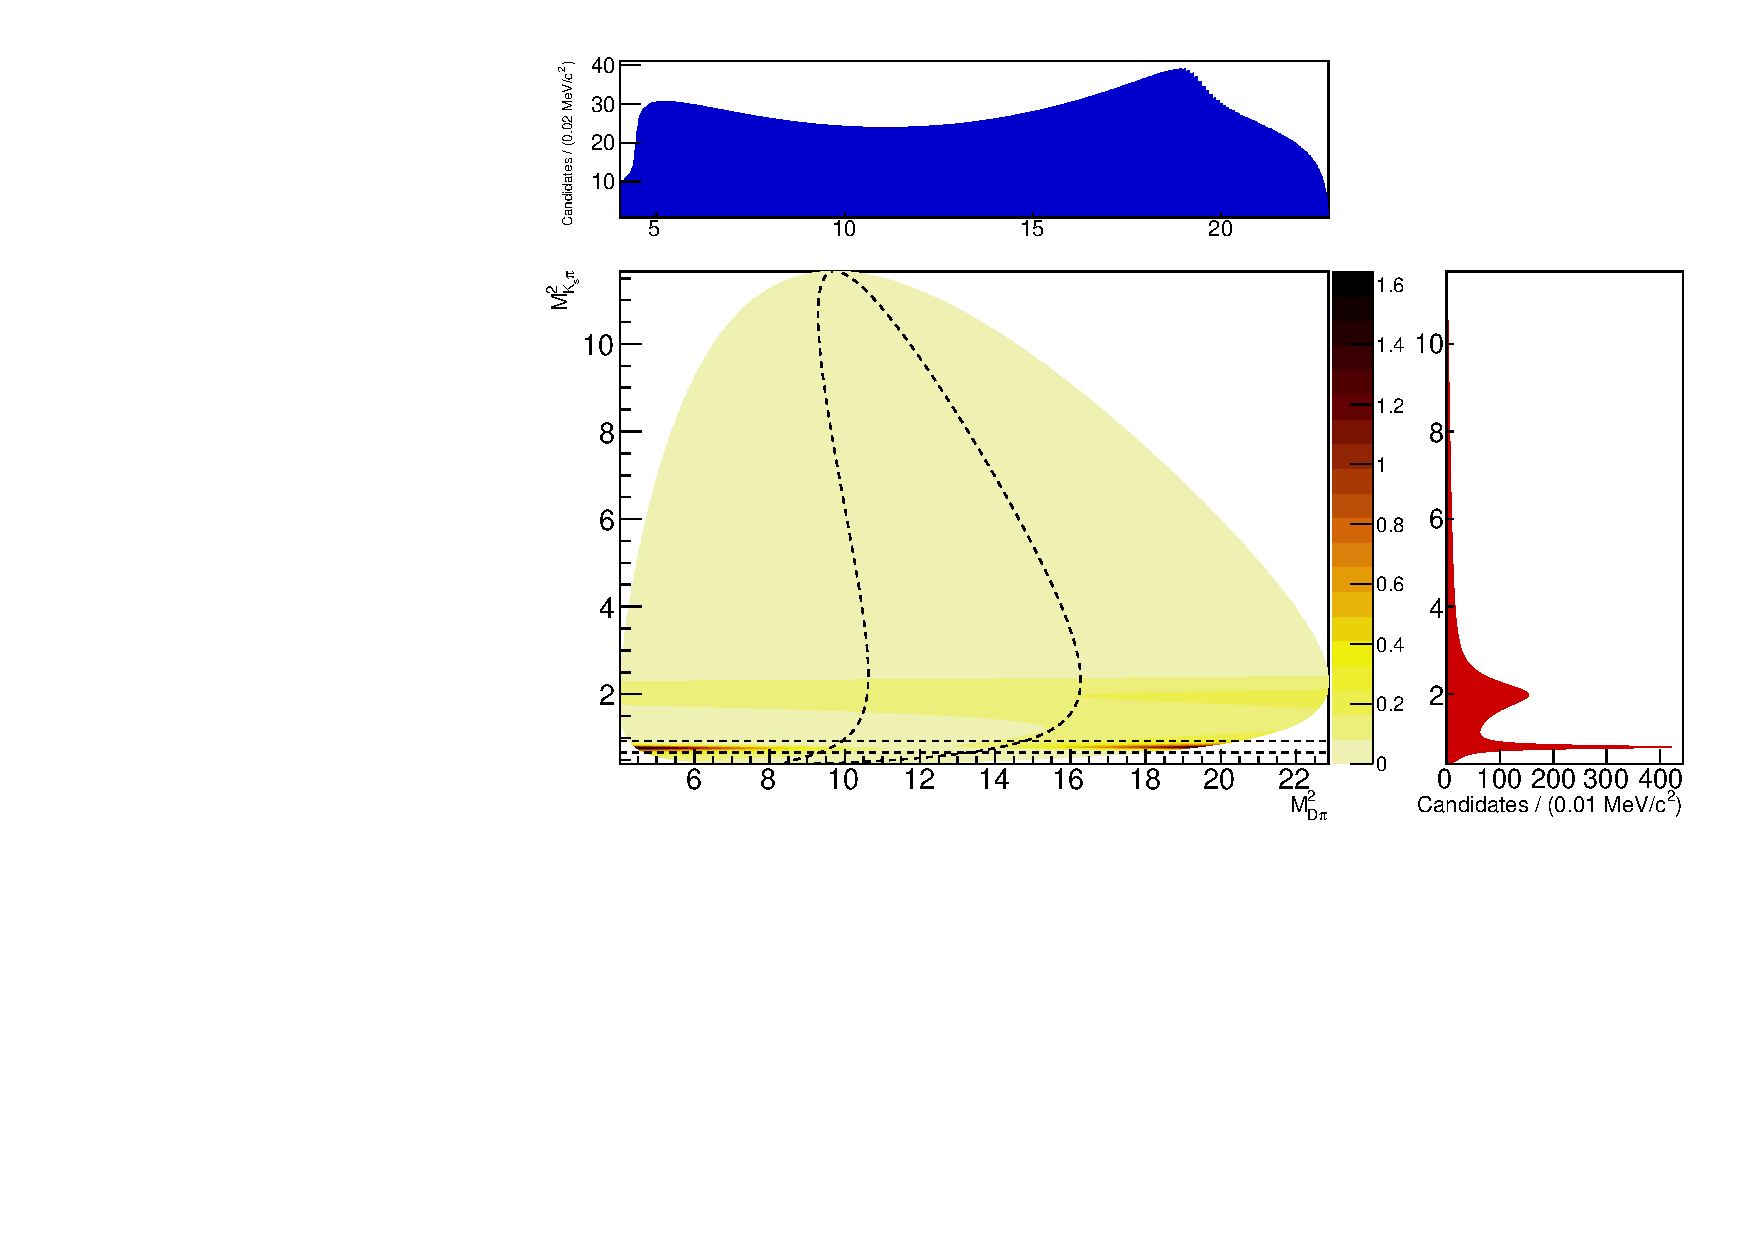
\includegraphics[width=\linewidth]{figures/results/dalitz.pdf}
\caption{An example amplitude model used in the estimate of $\kappa$. The horizontal axis labelled $M_{D\pi}^2$ is defined as $(p_D + p_{\pi})^2$, where $p_{X}$ is the four-momentum of particle $X$. Similarly, the vertical axis, labelled $M_{K_s\pi}^2$, is defined as $(p_{K_s} + p_{\pi})^2$. The projections in these two coordinates are shown. The $K^*(892)^+$ and $K^*(1430)^+$ resonances can be clearly seen in the red projection on the right hand side of the figure. The dashed lines on the plot represent the \Kstar mass and \KS helicity angle selection used in this analysis.}
\label{dalitzplot}
\end{figure}

\subsection{Estimation of the coherence factor, $\kappa$}
\label{sec:interpretation:kappa}

One thousand variants of the amplitude model, described in \sect\ref{sec:interpretation:model}, are generated, which differ in the amplitudes and phases of the components. For different variants of the amplitude model, the amplitudes and phases of the different resonances are varied randomly within limits; the limits for the amplitudes are given in \sect\ref{sec:interpretation:model} and all phases are generated randomly according to a uniform distribution between $-\pi$ and $\pi$. The masses and widths of the resonances are kept constant at their central values, given in \tab\ref{resonances}. 

For each model, $\kappa$ is computed according to the magnitude of the expression in \eqn\ref{kappadefinition}. This results in a distribution of $\kappa$ values estimated by the model, shown in \fig\ref{kappadistribution}. The mean and standard deviation of the resulting distribution provides an estimate of the central value and uncertainty of $\kappa$,  $0.95 \pm 0.04$. However, it is considered necessary to increase the uncertainty of this estimate in order to account for the skewness of the distribution, therefore a final value of $\kappa = 0.95 \pm 0.06$ is used in this thesis to extract the physics parameters of interest.

\begin{figure}[h]
\centering
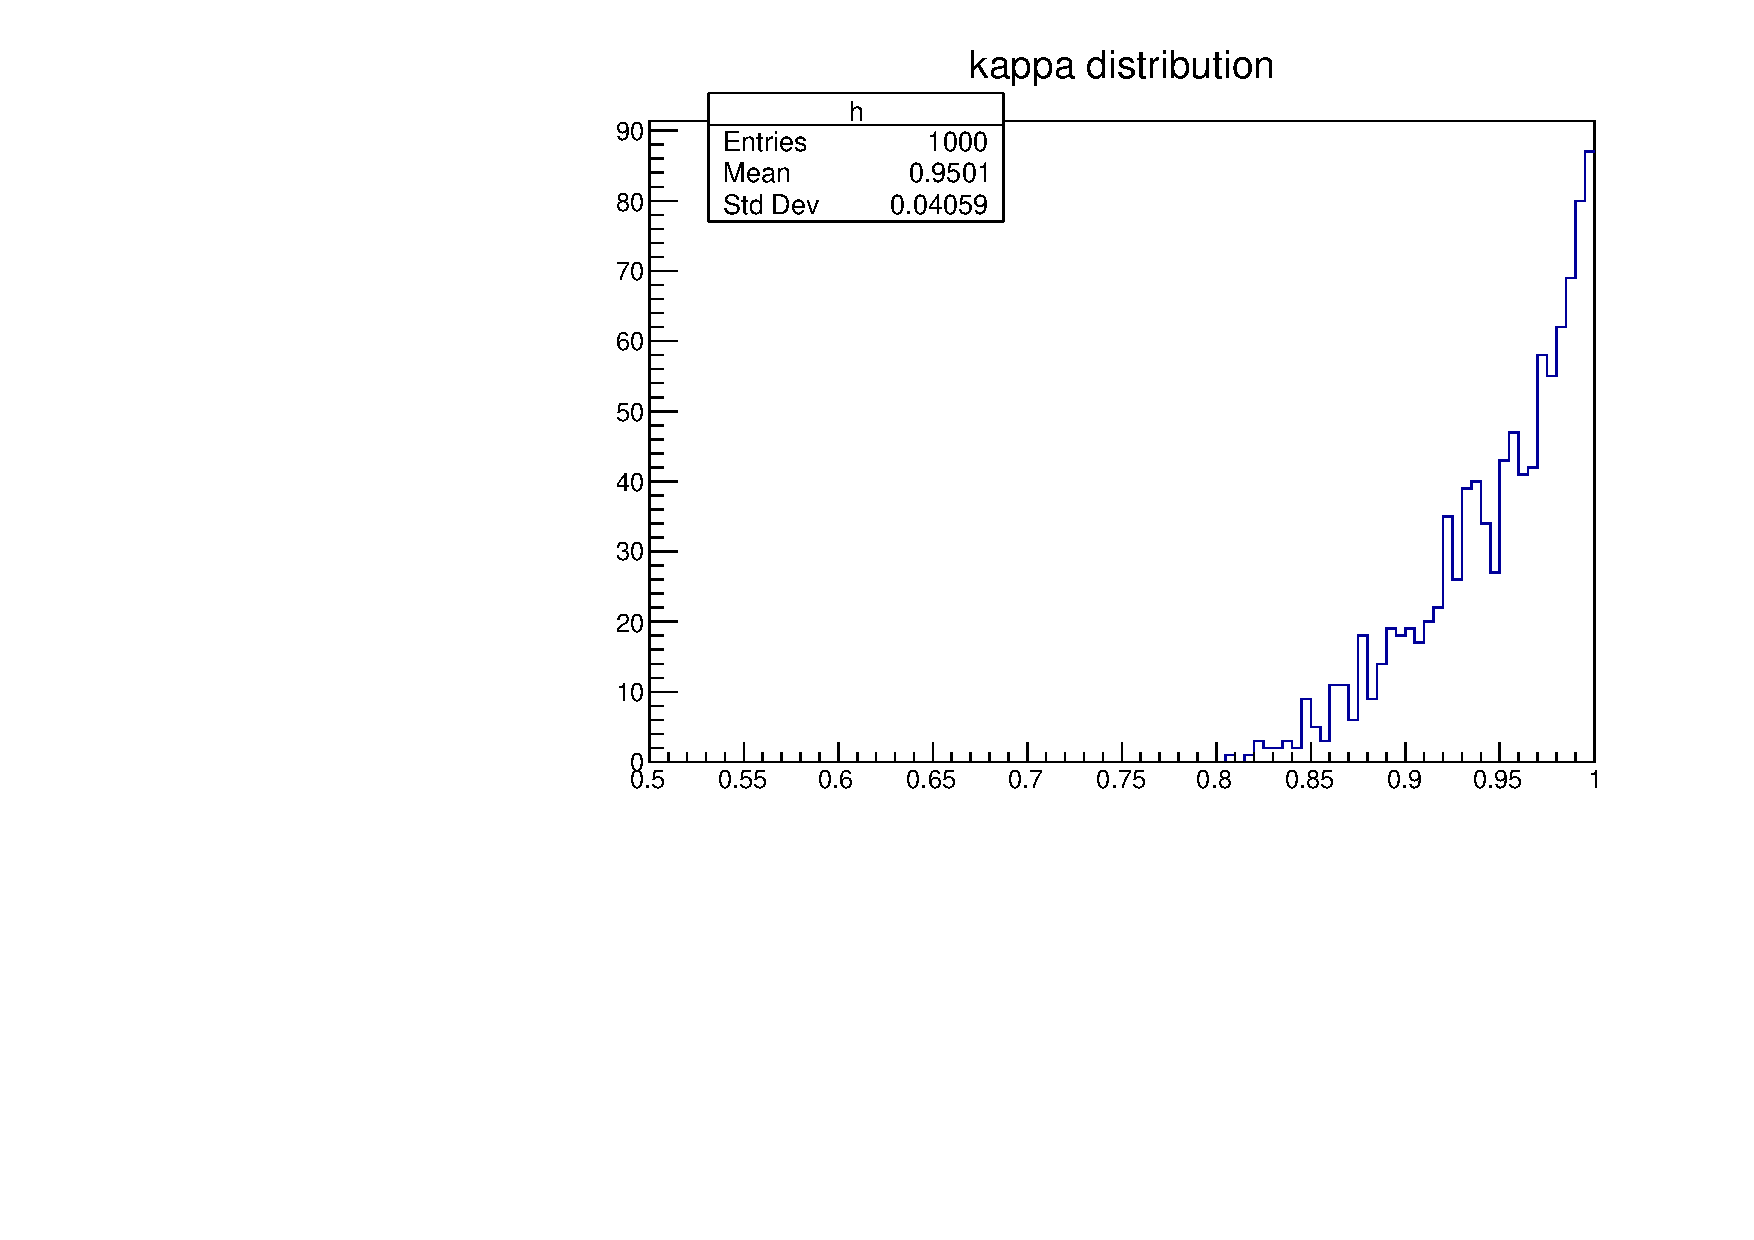
\includegraphics[trim = 0mm 0mm 0mm 8mm, clip, width=0.5\linewidth]{figures/results/kappa.pdf}
\caption{Distribution of the values of $\kappa$ from 1000 samples generated according to the amplitude model described in the text.}
\label{kappadistribution}
\end{figure}

\section{Four-body phase space acceptance variations}
\label{sec:interpretation:inputs}

For multibody \decay{\Dz}{\Kmp\pipm\pimp\pipm} and \decay{\Dz}{\pip\pim\pip\pim} decays, some regions of phase space may exhibit larger \CP violation than other regions. In this thesis, an inclusive analysis over phase space is performed. Therefore only the global \CP violation is elicited, and it may result in a loss of information of regional variation. The parameters $R_{K3\pi}$, $\delta_D^{K3\pi}$ and $F_{4\pi}$ allow the phase space to be treated inclusively, so that global asymmetries can be interpreted in a manner similar to the two-body \Dz decays.

The parameter $F_{4\pi}$ has been measured using data from CLEO~\cite{charm4pi}, while the values for $\delta_D^{K3\pi}$ and $R_{K3\pi}$ are taken from combining results from \lhcb and CLEO data~\cite{charmk3pi,charmk3pi_errata,LHCb-PAPER-2015-057}. These measurements have been corrected for a uniform efficiency across all phase space. When making measurements at \lhcb, the \lhcb acceptance leads to small non-uniformities in efficiency, which could enhance or diminish asymmetry in certain regions of phase space. In order to use the measurements of $F_{4\pi}$, $\delta_D^{K3\pi}$ and $R_{K3\pi}$ in this analysis these effects must be assessed and accounted for. This can be achieved either by correcting for the \lhcb yields under a scenario of uniform efficiency or by adjusting the $F_{4\pi}$, $\delta_D^{K3\pi}$ and $R_{K3\pi}$ parameters to match the \lhcb efficiency variation. The efficiencies calculated in \sect\ref{sec:cpfit:efficiencies} assume an average efficiency across the phase space. In order to correct for the \lhcb yields, event-wise efficiency corrections would have to be performed, which is not practical due to the large numbers of simulated events, and the computing power required. Therefore, consideration is given to whether the parameters $F_{4\pi}$, $\delta_D^{K3\pi}$ and $R_{K3\pi}$ require adjustment.

Figures~\ref{dalitzk3pi} and \ref{dalitz4pi} show projections of the four-body phase space distributions for \kpipipi and \pipipipi modes respectively. These plots are comparisons of distributions using simulated generator-level signal events without any acceptance effects, and fully-reconstructed simulated signal events used in this analysis. It can be seen that the distributions are very similar, suggesting that any differences due to \lhcb acceptance effects are very small. This implies that $R_{K3\pi}$, $\delta_D^{K3\pi}$ and $F_{4\pi}$ can be used directly in the interpretation of \lhcb results.

\begin{figure}[h]
\centering
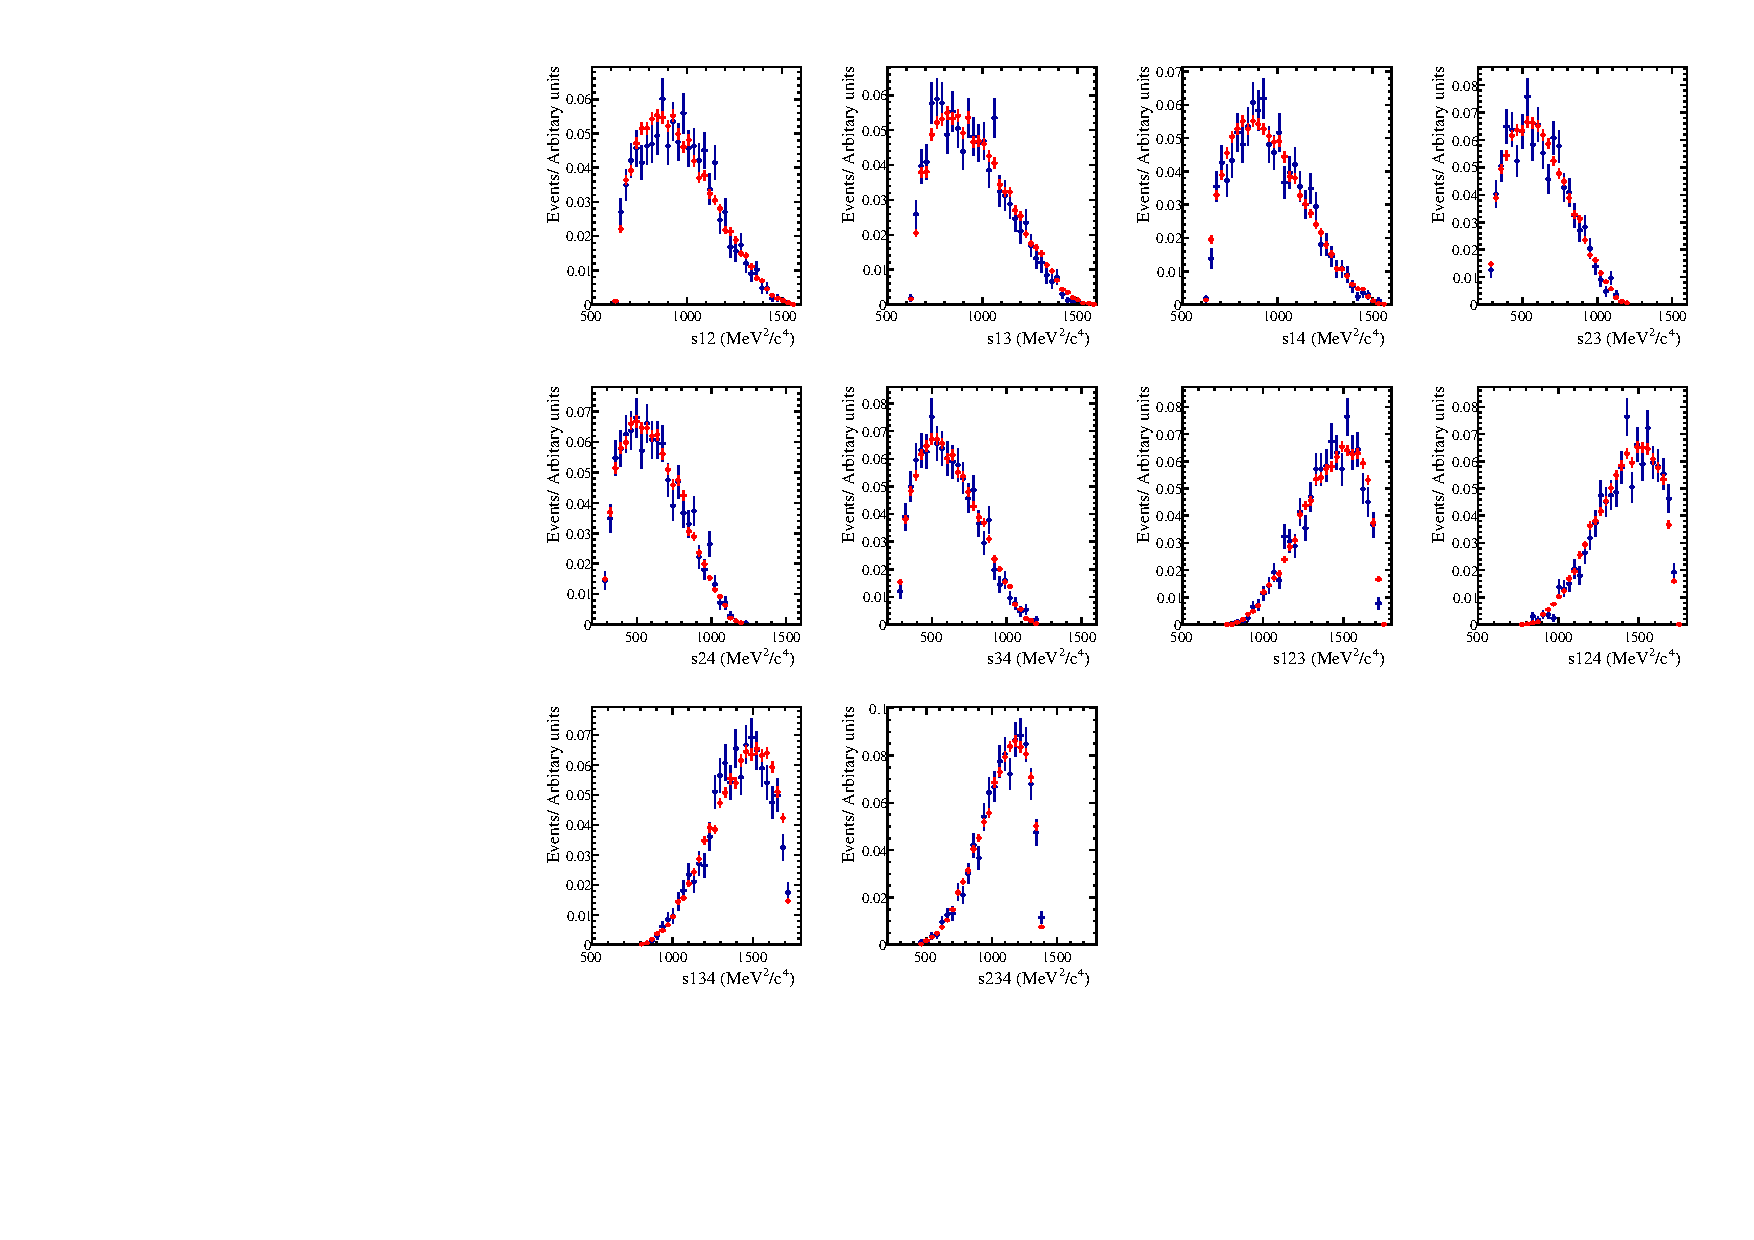
\includegraphics[width=0.9\linewidth]{figures/results/dalitzDist_KPiPiPi.pdf}
\caption{Distributions of invariant mass squared for all combinations of two- and three-particles from the four \Dz daughters with simulated generator level events (blue) and fully reconstructed and selected events (red) in the \kpipipi mode. The variable $sXY$ is defined as $(p_X + p_Y)^2$, where $X$ and $Y$ represent labels that refer to a specific daughter of the \Dz meson, and $p_X$ is the four-momentum of particle $X$. The \Dz daughter labels are defined by: \decay{\Bm}{\D(K^-_1\pi^+_2\pi^-_3\pi^+_4)\Kstarm}.}
\label{dalitzk3pi}
\end{figure}

\begin{figure}[h]
\centering
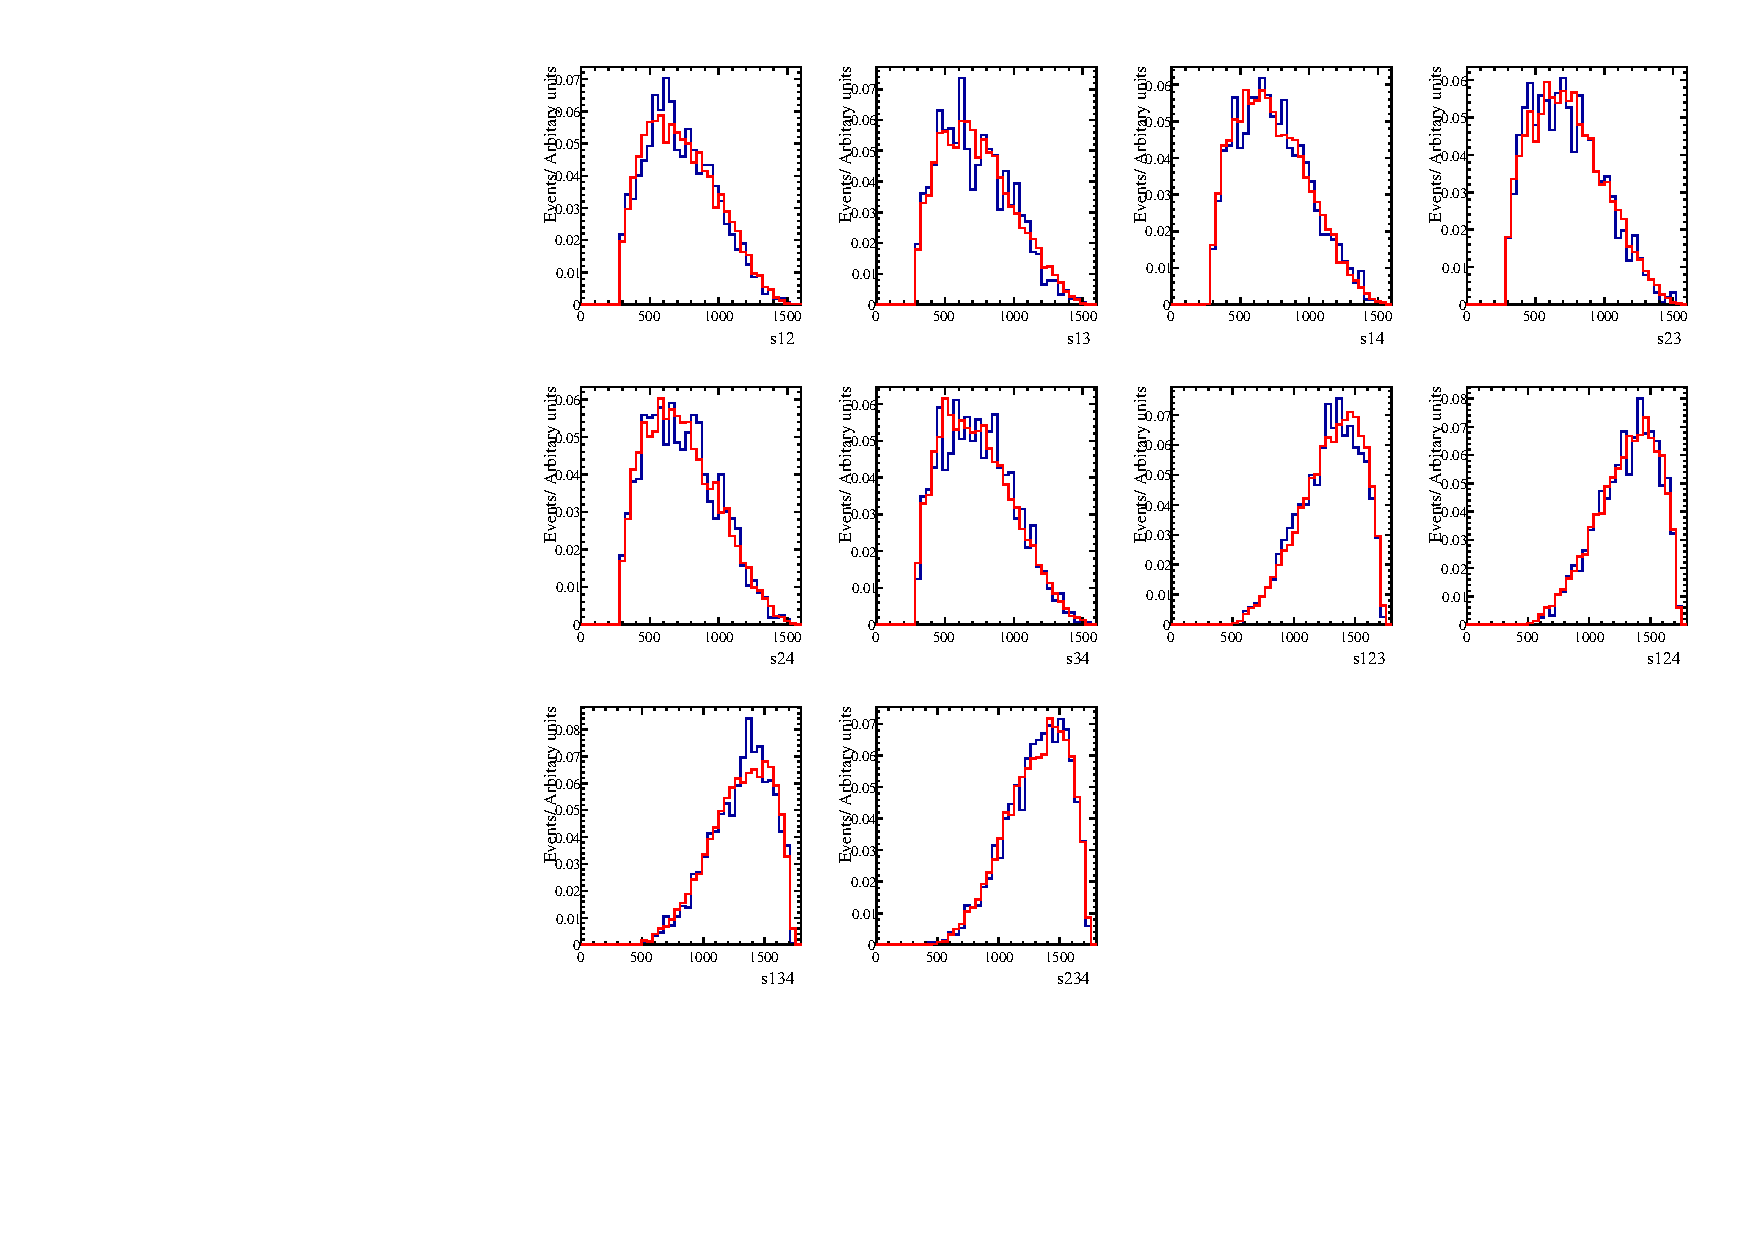
\includegraphics[width=0.9\linewidth]{figures/results/dalitzDist_PiPiPiPi.pdf}
\caption{Distributions of invariant mass squared for all combinations of two- and three-particles from the four \Dz daughters with simulated generator level events (blue) and fully reconstructed and selected events (red) in the \pipipipi mode. The variable $sXY$ is defined as $(p_X + p_Y)^2$, where $X$ and $Y$ represent labels that refer to a specific daughter of the \Dz meson, and $p_X$ is the four-momentum of particle $X$. The \Dz daughter labels are defined by: \decay{\Bm}{\D(\pi^-_1\pi^+_2\pi^-_3\pi^+_4)\Kstarm}.}
\label{dalitz4pi}
\end{figure}

To verify the above implication, further studies are performed to assess whether the values of the parameters $R_{K3\pi}$ and $\delta_D^{K3\pi}$ require any corrections for the determination of the physics parameters. To assess the effects of any small variations in the four-body phase space for \kpipipi decays, the coherence factor and strong phase are calculated from a preliminary version of the \decay{\Dz}{\Km\pip\pim\pip} amplitude model described in Ref.~\cite{LHCb-PAPER-2017-040}, both under the assumptions of uniform acceptance and including \lhcb acceptance corrections. This study was possible as the \decay{\Dz}{\Km\pip\pim\pip} amplitude model was already being developed for a different purpose. The differences between the two scenarios give an estimate of the corrections that should be applied to $R_{K3\pi}$ and $\delta_D^{K3\pi}$. The corresponding differences are calculated to be 0.002 for the coherence factor and 0.7$^{\circ}$ for the strong phase difference, compared to the input values of $R_{K3\pi} = 0.43^{+0.17}_{-0.13}$ and $\delta_D^{K3\pi} = \left(128^{+28}_{-17}\right)$. Therefore, the size of the corrections due to the \lhcb phase space acceptance are negligible in comparison to the CLEO-c/LHCb uncertainties. Hence no further corrections are made. 

A similar study for \decay{\Dz}{\pim\pip\pim\pip} was not possible as a reliable model was unavailable at the time.~\footnote{A \decay{\Dz}{\pim\pip\pim\pip} amplitude model based on CLEO data has subsequently been published~\cite{4piamplitude}.} Therefore, the value of $F_{4\pi}$ is taken directly from the CLEO-c measurement, $0.734 \pm 0.028$~\cite{charm4pi}, assuming that any correction would be negligible with respect to the measurement uncertainty as is the case for $R_{K3\pi}$ and $\delta_D^{K3\pi}$. 

\section{Results in terms of $r_B$, $\delta_B$ and \Pgamma}
\label{sec:interpretation:gammadini}

The \CP observables, measured in the \CP fit and listed in \sect\ref{sec:cpfit:summary}, can be used to extract information on the physics parameters of interest: $r_B$, $\delta_B$ and \Pgamma, via \eqns~\ref{exp_Acp} - \ref{exp_Rpm4body}. The values of the coherence factor $\kappa$, estimated in \sect\ref{sec:interpretation:coherence}, and the parameters $r_D^{K\pi}$, $\delta_D^{K\pi}$, $r_D^{K3\pi}$, $\delta_D^{K3\pi}$, $R_{K3\pi}$ and $F_{4\pi}$, taken from Ref.~\cite{HFAG,charmk3pi,charmk3pi_errata,LHCb-PAPER-2015-057,charm4pi}, are required as inputs. The set of parameters $\kappa$, $r_D^{K\pi}$, $\delta_D^{K\pi}$, $r_D^{K3\pi}$, $\delta_D^{K3\pi}$, $R_{K3\pi}$ and $F_{4\pi}$, here referred to as $\mathbb{P}$, are constrained to the values given in \tab\ref{inputparameters}, which is common in the analysis of \lhcb measurements. Constraining these parameters, rather than fixing them to their central values, allows the possibility of the \CP observables providing additional sensitivity\footnote{For the analysis presented in this thesis, the dataset is too small to have an impact on the sensitivity of $\mathbb{P}$.} to $\mathbb{P}$.

The sensitivity of the data to the set of physics parameters $r_B$, $\delta_B$ and \Pgamma is extracted using the $\chi^2$ minimisation procedure described below. The data used are the measured \CP observables, $\mathbf{x_m}$, along with their combined statistical and systematic covariance matrix $V_0$. The model, expressed by \eqns~\ref{exp_Acp} - \ref{exp_Rpm4body}, is used to calculate \CP observables, $\mathbf{x}(\rb, \deltab, \Pgamma)$, from the set of constrained parameters $\mathbb{P}$ for different values of the physics parameters \rb, \deltab and \Pgamma. The $\chi^2$ minimisation procedure is performed, taking correlations into account, with
\begin{equation}
\chisq(\rb, \deltab, \Pgamma) = (\mathbf{x}(\rb, \deltab, \Pgamma) - \mathbf{x_m})^TV_0^{-1}(\mathbf{x}(\rb, \deltab, \Pgamma) - \mathbf{x_m}) \text{ .}
\end{equation}
The \chisq is calculated at various points in $\left(\rb, \deltab, \Pgamma\right)$ space, and the position of the global minimum, $\chisq_{\text{min}}$, represents the point corresponding to the best estimates for the central values of these parameters. The difference between the \chisq value at each point and that of the global minimum value, $\Delta\chisq(\rb, \deltab, \Pgamma) = \chisq(\rb, \deltab, \Pgamma) - \chisq_{\text{min}}$, can quantify the confidence in the global minimum, and the gradient of $\Delta\chisq$ in the direction of a given parameter reveals the sensitivity of the data to that parameter. The \chisq value at the global minimum is 3.0 with 9 degrees of freedom. The confidence level for any pair of parameters is calculated assuming that these are normally distributed, which enables the $\Delta\chisq = 2.30,\ 6.18,\ \text{and } 11.8$ contours to be drawn, corresponding to 68.3\%, 95.5\%, \text{and} 99.7\% confidence levels respectively.

\begin{table}
\centering
\begin{tabular}{cc}
Fit parameter & Value \\
\hline
$\kappa$ & $0.96 \pm 0.06$ \\
$r_D^{K\pi}$ & $0.0591 \pm 0.0003$ \\
$\delta_D^{K\pi}$ & $191.8 \pm 12.1$ \\
$r_D^{K3\pi}$ & $0.0549 \pm 0.0006$ \\
$\delta_D^{K3\pi}$ & $128 \pm 28$ \\
$R_{K3\pi}$ & $0.43 \pm 0.17$ \\
$F_{4\pi}$ & $0.737 \pm 0.028$
\end{tabular}
\caption{Values of the external inputs used as constraints. These values are taken from Ref.~\cite{HFAG,charmk3pi,charmk3pi_errata,charm4pi}.}
\label{inputparameters}
\end{table}

Figures~\ref{gammadiniplots2body} and \ref{gammadiniplotsallmodes} depict 2D contour plots of $r_B$ versus \Pgamma and $\delta_B$ versus \Pgamma. \Fig\ref{gammadiniplots2body} shows the contour plots using the \CP observables from the two-body modes only and \fig\ref{gammadiniplotsallmodes} shows the contour plots using the \CP observables from both the two- and four-body decays. The addition of the four-body modes improves the constraints on the physics parameters and provides additional distinction between the two minima. 

The data are consistent with the value of $\gamma$ indicated by previous measurements~\cite{LHCb-PAPER-2016-032, CKMFitter}, $\sim 70^\circ$. The values of $r_B$, $\delta_B$ and \Pgamma are determined at the point where the global minimum value of $\chi^2$ is found. The value of \rb is calculated to be $r_B = 0.113^{+0.017}_{-0.019}$. The parameter \deltab has a measured central value of $43^{\circ}$ with a $1\sigma$ confidence interval of $[24, 62]^{\circ}$, and $2\sigma$ confidence intervals of $[9, 84]^{\circ}$ and $[103,173]^{\circ}$. The central value of \Pgamma is measured to be $41^{\circ}$ with a $1\sigma$ confidence interval of $[25, 58]^{\circ}$, and $2\sigma$ confidence intervals of $[10, 87]^{\circ}$ and $[97,167]^{\circ}$. No value of \Pgamma or \deltab is excluded at the $3\sigma$ level. These results provide the current best sensitivity to the hadronic parameters of the \Bm decay, \rb and \deltab.

\begin{figure}[h]
\centering
\subfloat[$r_B$ versus \Pgamma]{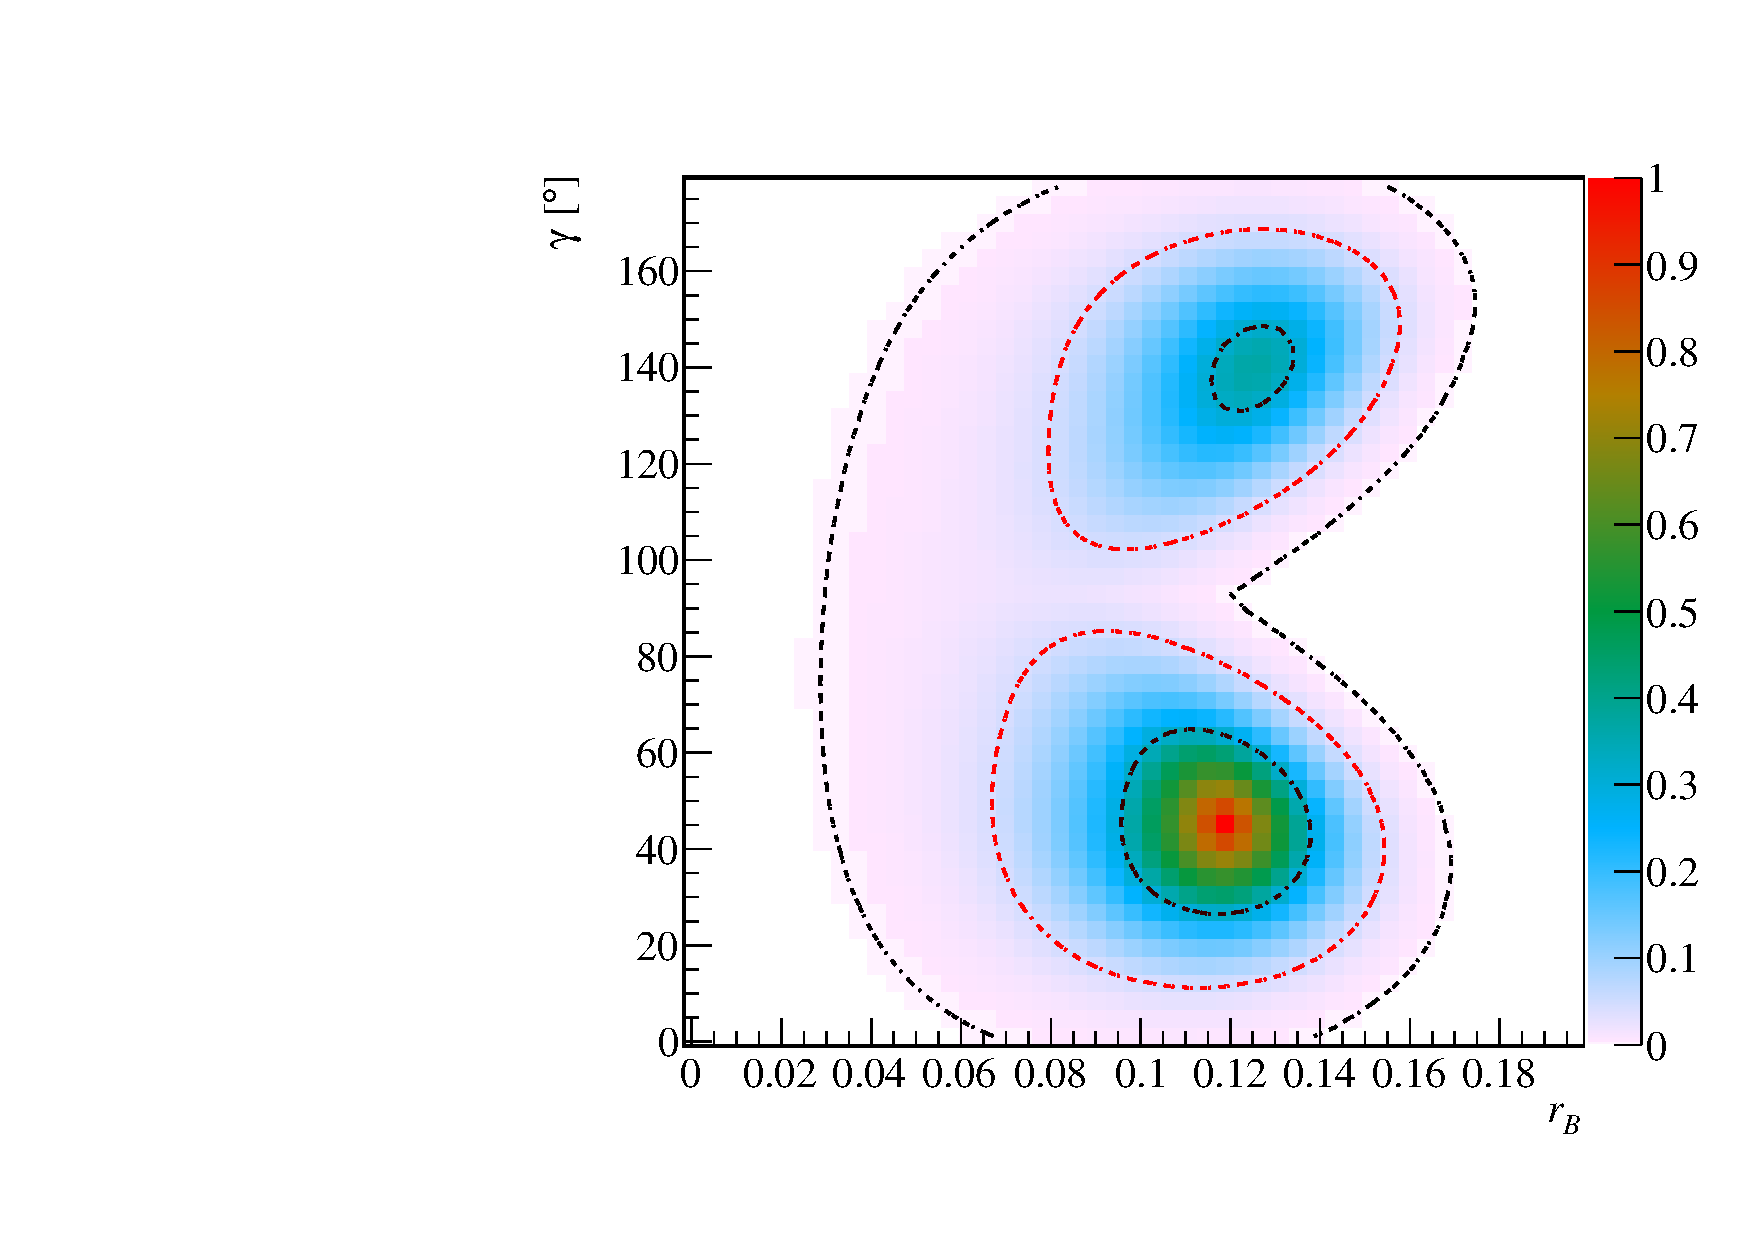
\includegraphics[width=0.5\linewidth]{figures/interpretation/rBu_dkstar_gamma_2Dscan_nomixing_2body.pdf}}
\subfloat[$\delta_B$ versus \Pgamma]{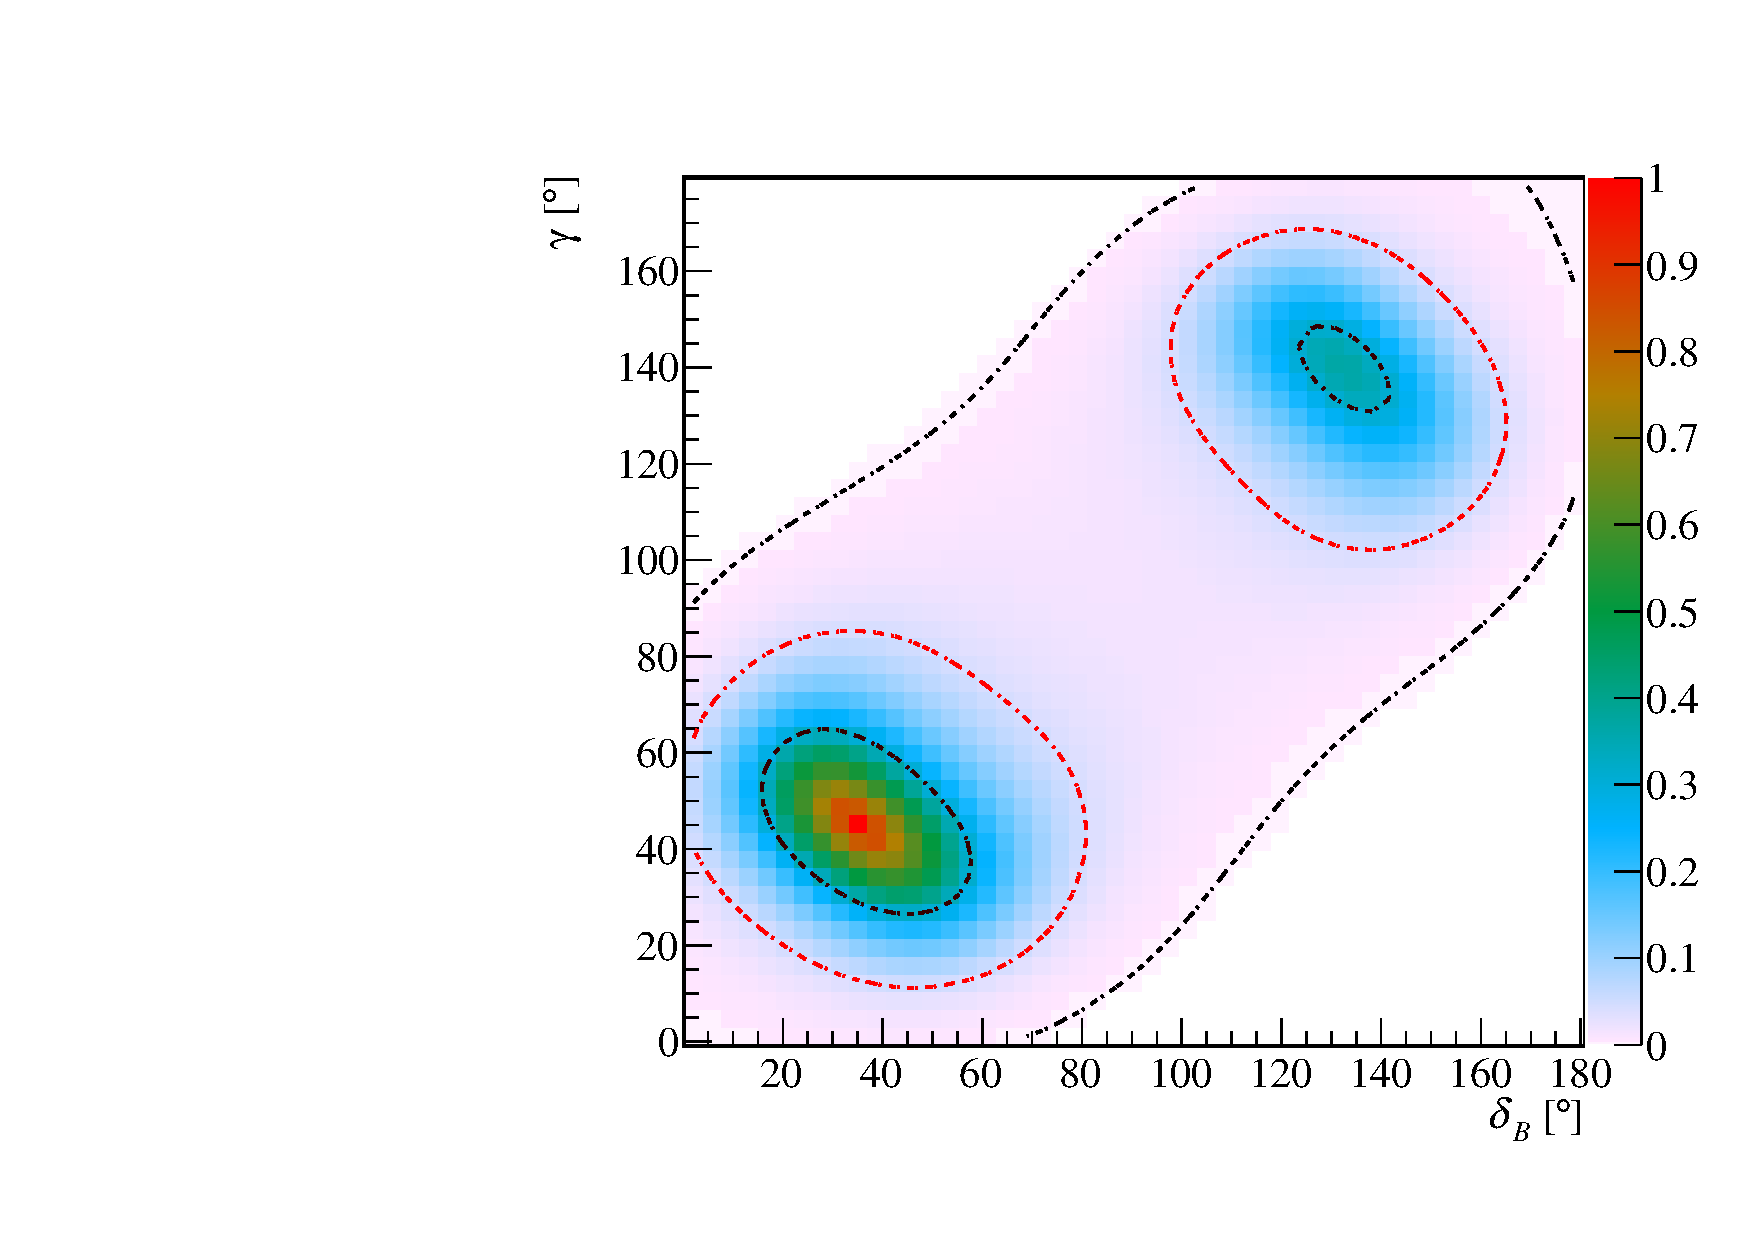
\includegraphics[width=0.5\linewidth]{figures/interpretation/deltaBu_dkstar_gamma_2Dscan_nomixing_2body.pdf}}
\caption{Contour plots showing 2D scans of the physics parameters using the two-body \Dz decay modes only. The dashed lines represent the $\Delta \chi^2 = 2.30,\ 6.18,\ \text{and } 11.8$ contours, corresponding to 68.3\%, 95.5\%, and 99.7\% confidence levels (CL), respectively. The colour scale represents $(1 - \text{CL})$.}
\label{gammadiniplots2body}
\end{figure}

\begin{figure}[h]
\centering
\subfloat[$r_B$ versus \Pgamma]{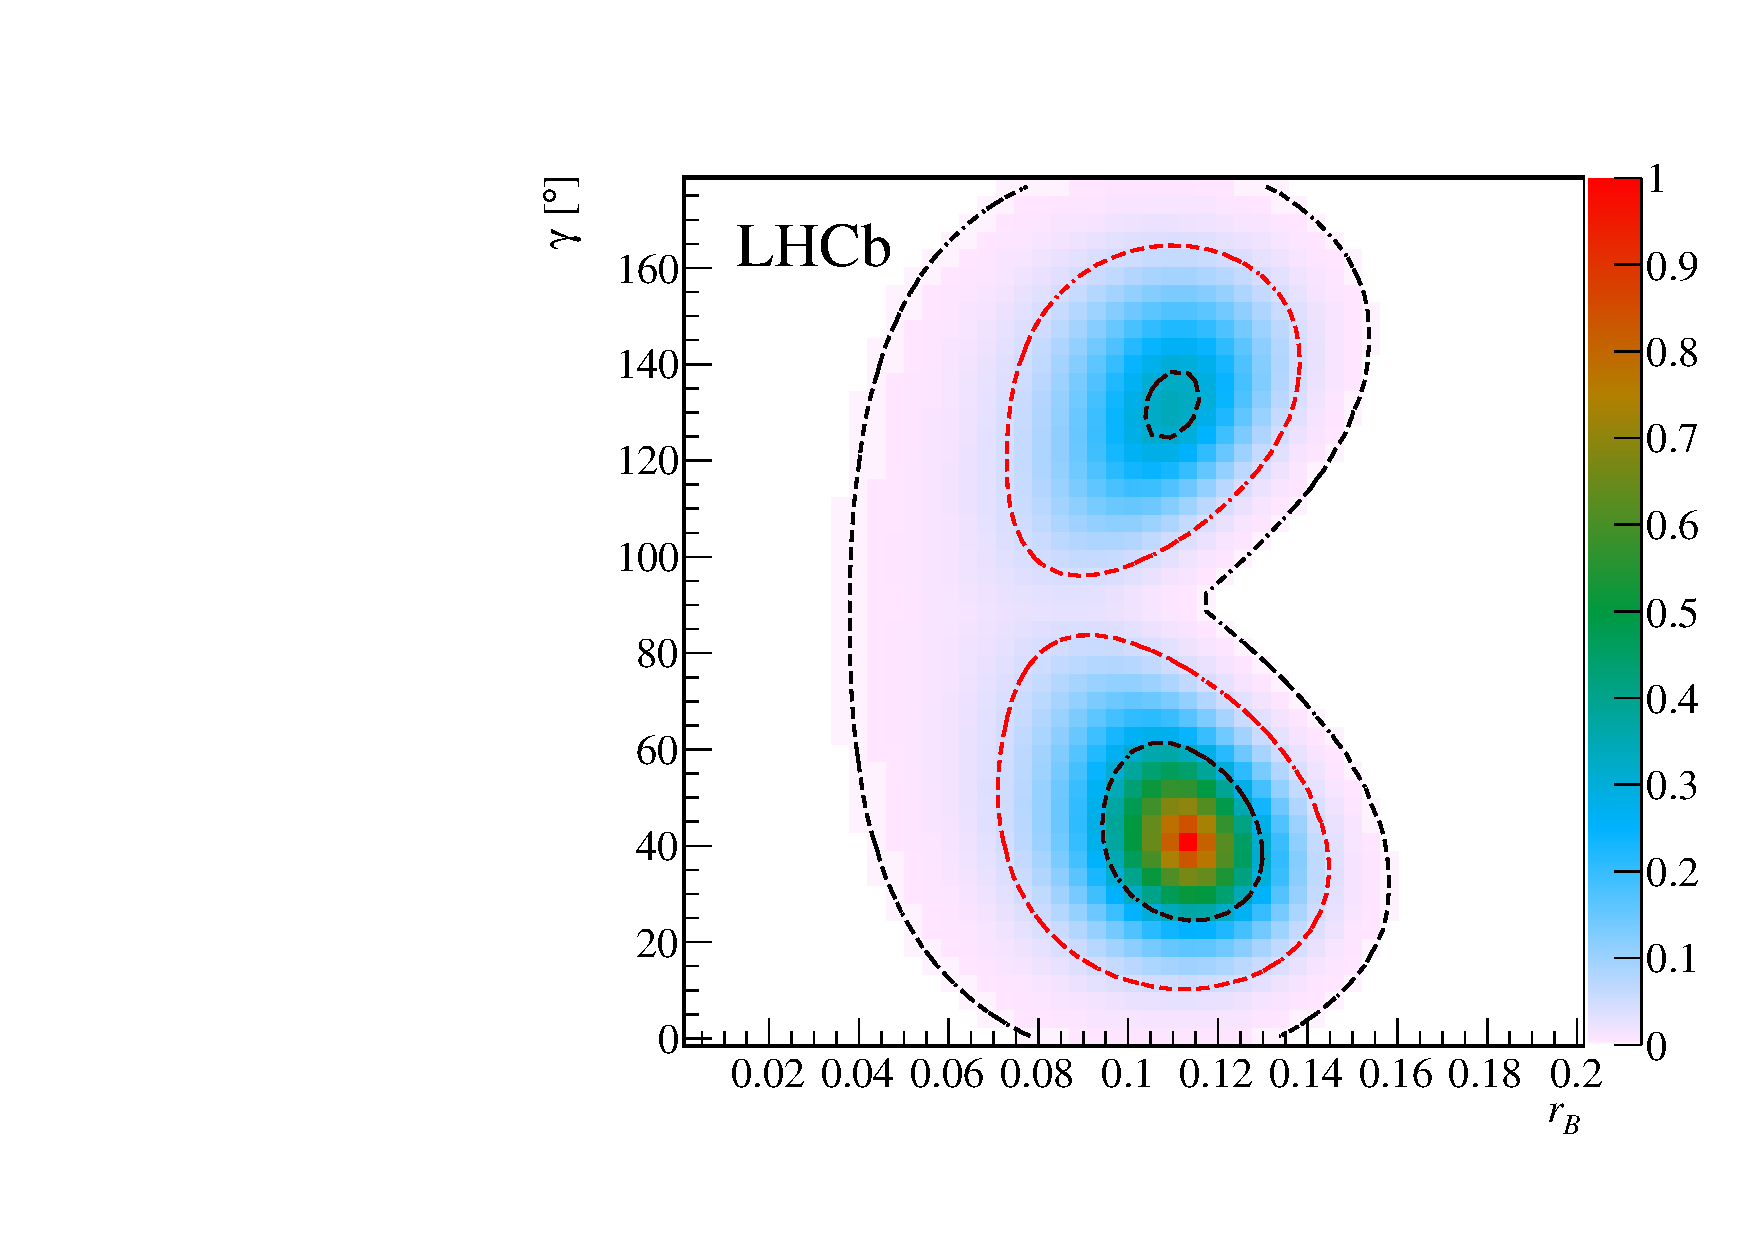
\includegraphics[width=0.5\linewidth]{figures/interpretation/rBu_dkstar_gamma_2Dscan_nomixing_all.pdf}}
\subfloat[$\delta_B$ versus \Pgamma]{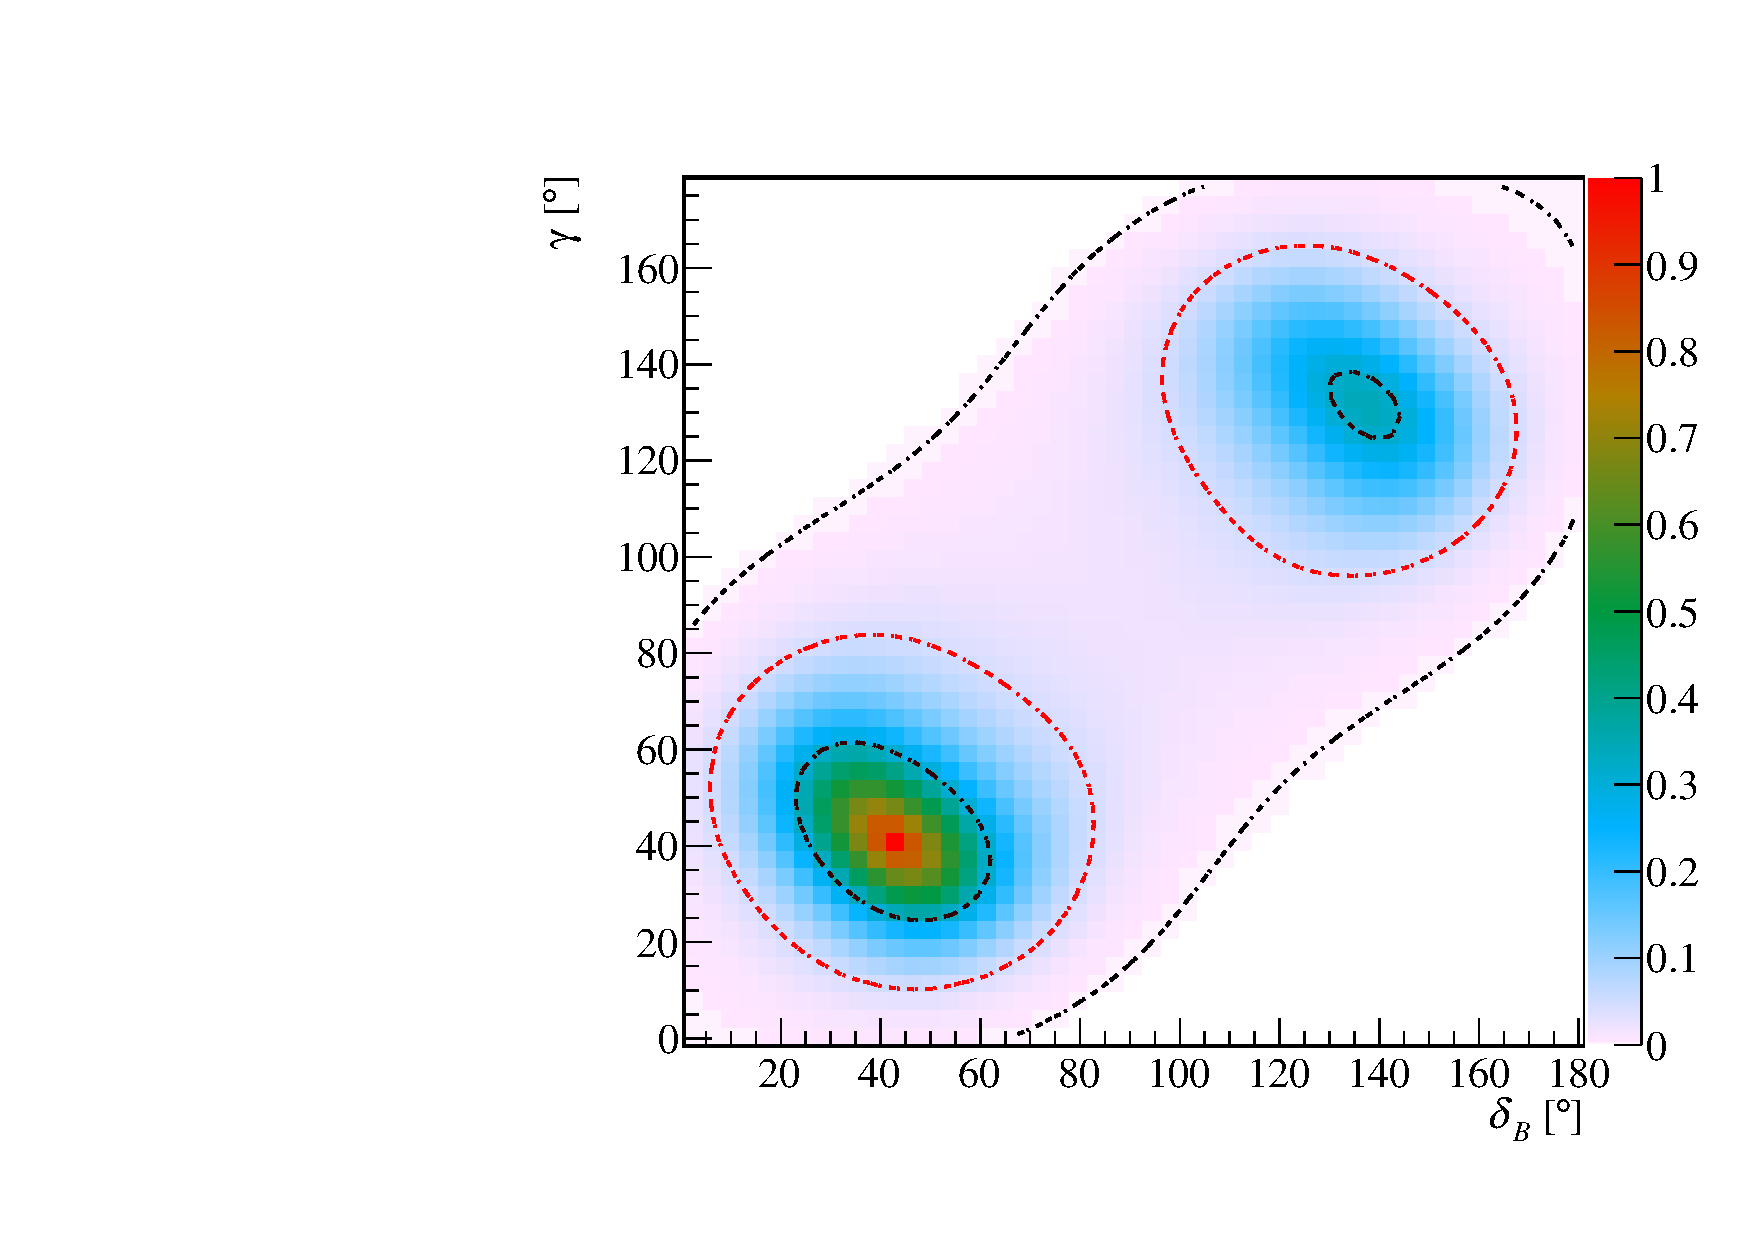
\includegraphics[width=0.5\linewidth]{figures/interpretation/deltaBu_dkstar_gamma_2Dscan_nomixing_all.pdf}}
\caption{Contour plots showing 2D scans of the physics parameters using both the two- and four-body \Dz decay modes. The dashed lines represent the $\Delta \chi^2 = 2.30,\ 6.18,\ \text{and } 11.8$ contours, corresponding to 68.3\%, 95.5\%, and 99.7\% CL, respectively. The colour scale represents $(1 - \text{CL})$.}
\label{gammadiniplotsallmodes}
\end{figure}

\section{Expected future sensitivity to $r_B$, $\delta_B$ and \Pgamma using \btodkst decays}
\label{sec:interpretation:futuresensitivity}

In this thesis, the \btodkst mode has shown an increase of three times the yield per unit integrated luminosity from \runone to \runtwo, mainly due to the increase in centre of mass energy of the $pp$ collisions from 7 and 8~\tev to 13~\tev. As previously stated, the data used in this analysis were collected in 2011 and 2012, forming the \runone \dataset, and 2015 and 2016, forming part of the \runtwo \dataset. The current running period of the LHC, namely \runtwo, is ongoing until the end of 2018. Run 3, the next running period, is planned to take place between 2021 and 2023.

The projected final yields for Run 2 and Run 3 are estimated using the forecasts for the integrated luminosity and expected improvements in the detector performance during these data-taking periods. The projections of the integrated luminosities can be found in \tab\ref{projectedyields}. It is assumed that the yield per unit integrated luminosity remains the same for duration of \runtwo since no significant changes to the detector or running conditions are expected. Between Run 2 and Run 3 the detector will undergo an upgrade to improve detector performance, its trigger and event reconstruction. This will include moving to a fully software-based trigger~\cite{CERN-LHCC-2014-016} and the rebuilding of many detector components, which will allow the experiment to run at an instantaneous luminosity of $2 \times 10^{33}~\text{cm}^{-2}\text{s}^{-1}$, a five-fold increase on the current conditions~\cite{CERN-LHCC-2014-016}. Additionally, the centre of mass energy is expected to increase to 14~\tev. Therefore, Run 3 is expected to produce a minimum of 5~\invfb per year for three years~\cite{CERN-LHCC-2014-016}. The upgrade to a fully software-based trigger also improves the trigger efficiencies for the fully hadronic modes by about a factor of two compared to \runone~\cite{CERN-LHCC-2014-016}. Overall, yields of \B meson decay modes in Run 3 are expected to increase by a factor of $\sim$32 compared to \runone, even before any potential improvements in the analysis procedure. The result of these assumptions are shown in the projected yield estimates in \tab\ref{projectedyields}.

\begin{table}
\resizebox{\textwidth}{!}{
\begin{tabular}{cccc}
\hline
Year & Integrated Luminosity & \kpi yield & Yield per \invfb \\
\hline
\runone & 3\invfb & 725 & 242 \\
\runtwo (up to 2016) & 1.8\invfb & 1390 & 771 \\
\textbf{Run 2 (after 2016)} & \textbf{3.2\invfb} & \textbf{2466} & \textbf{771} \\
\textbf{Run 3} & \textbf{15\invfb} & \textbf{23130} & \textbf{1542} \\
\hline
\end{tabular}}
\caption{Yields and projected yields for the data-taking periods of the LHC. The entries in bold are projected yields, whereas the other entries refer to data used in this thesis. Projected results are justified in the text, with information taken from Ref.~\cite{CERN-LHCC-2014-016}.}
\label{projectedyields}
\end{table}

% Luminosity/Yield factor for Run 2: 2.2
% Luminosity/Yield factor for Run 3: 13.1

Using the results of \tab\ref{projectedyields}, the projected sensitivity to the physics parameters \rb, \deltab and \Pgamma are estimated, assuming conservatively that the systematic uncertainties remain the same. \Fig\ref{gammadiniplotsrun2} gives the projected results at the end of Run 2 as 2D contour plots of \rb versus \Pgamma and \deltab versus \Pgamma. The equivalent plots for the end of Run 3 are shown in \fig\ref{gammadiniplotsrun3}. 

\begin{figure}[h]
\centering
\subfloat[\rb versus \Pgamma]{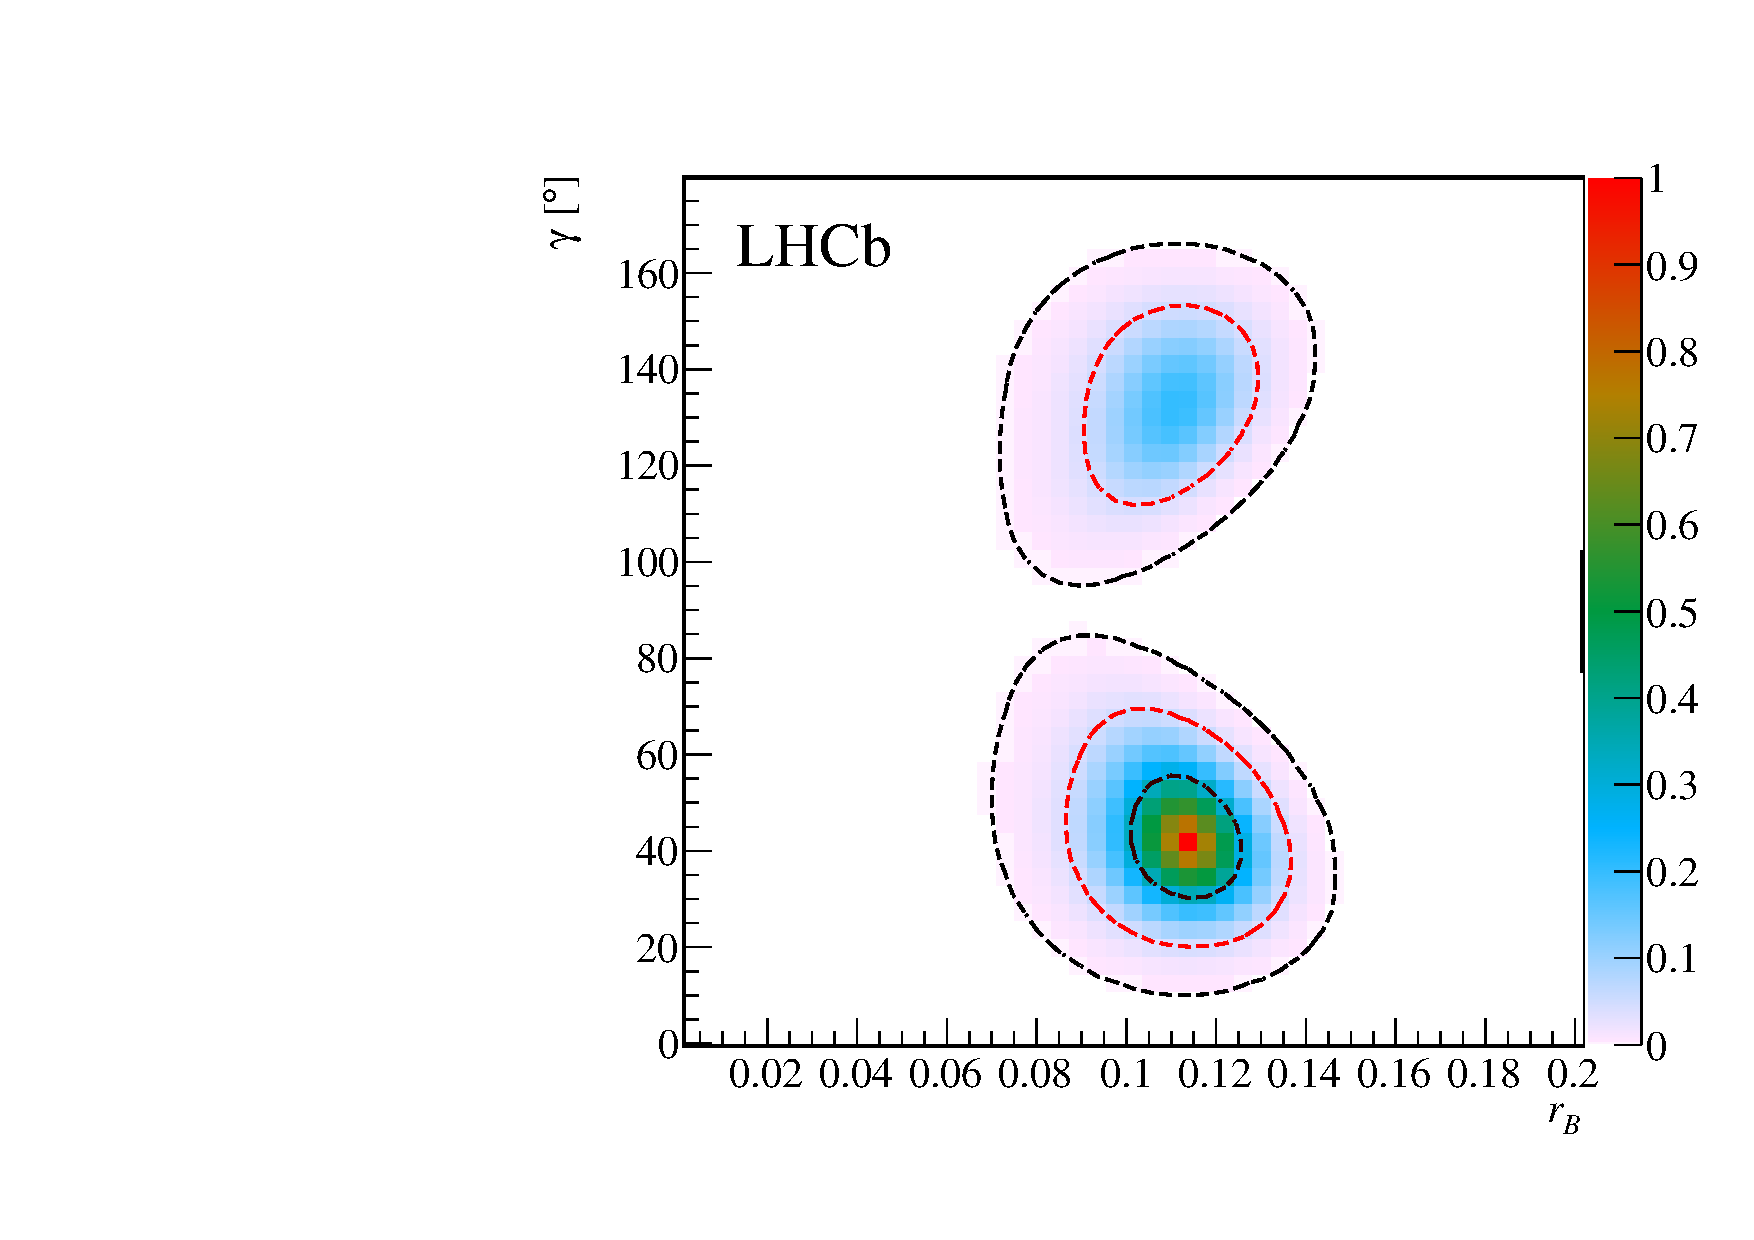
\includegraphics[width=0.5\linewidth]{figures/interpretation/rBu_dkstar_gamma_2Dscan_nomixing_Run2.pdf}}
\subfloat[\deltab versus \Pgamma]{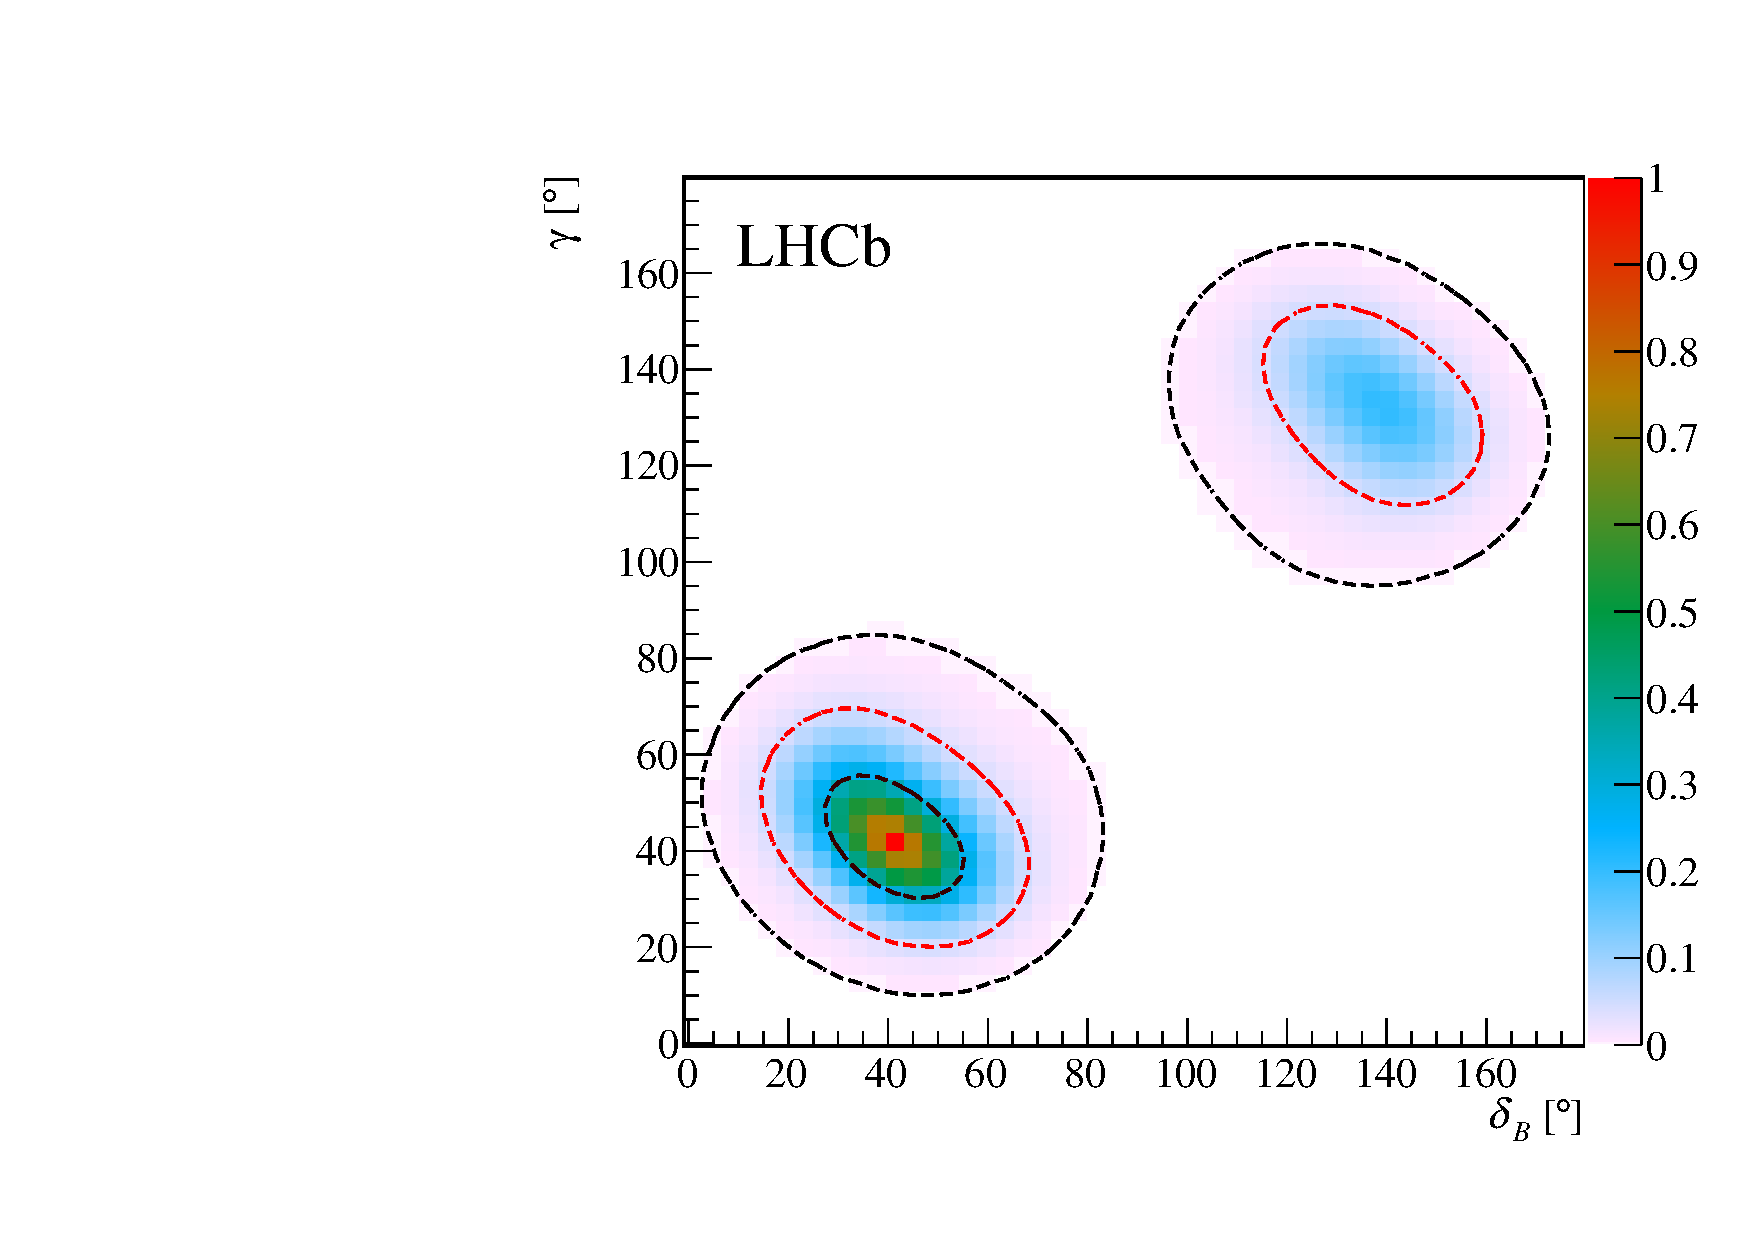
\includegraphics[width=0.5\linewidth]{figures/interpretation/deltaBu_dkstar_gamma_2Dscan_nomixing_Run2.pdf}}
\caption{Contour plots showing projected 2D scans of the physics parameters measured in \btodkst decays at the end of \runtwo, assuming the central values remain the same. The dashed lines represent the $\Delta \chi^2 = 2.30,\ 6.18,\ \text{and } 11.8$ contours, corresponding to 68.3\%, 95.5\%, and 99.7\% CL, respectively. The colour scale represents $(1 - \text{CL})$.}
\label{gammadiniplotsrun2}
\end{figure}

\begin{figure}[h]
\centering
\subfloat[\rb versus \Pgamma]{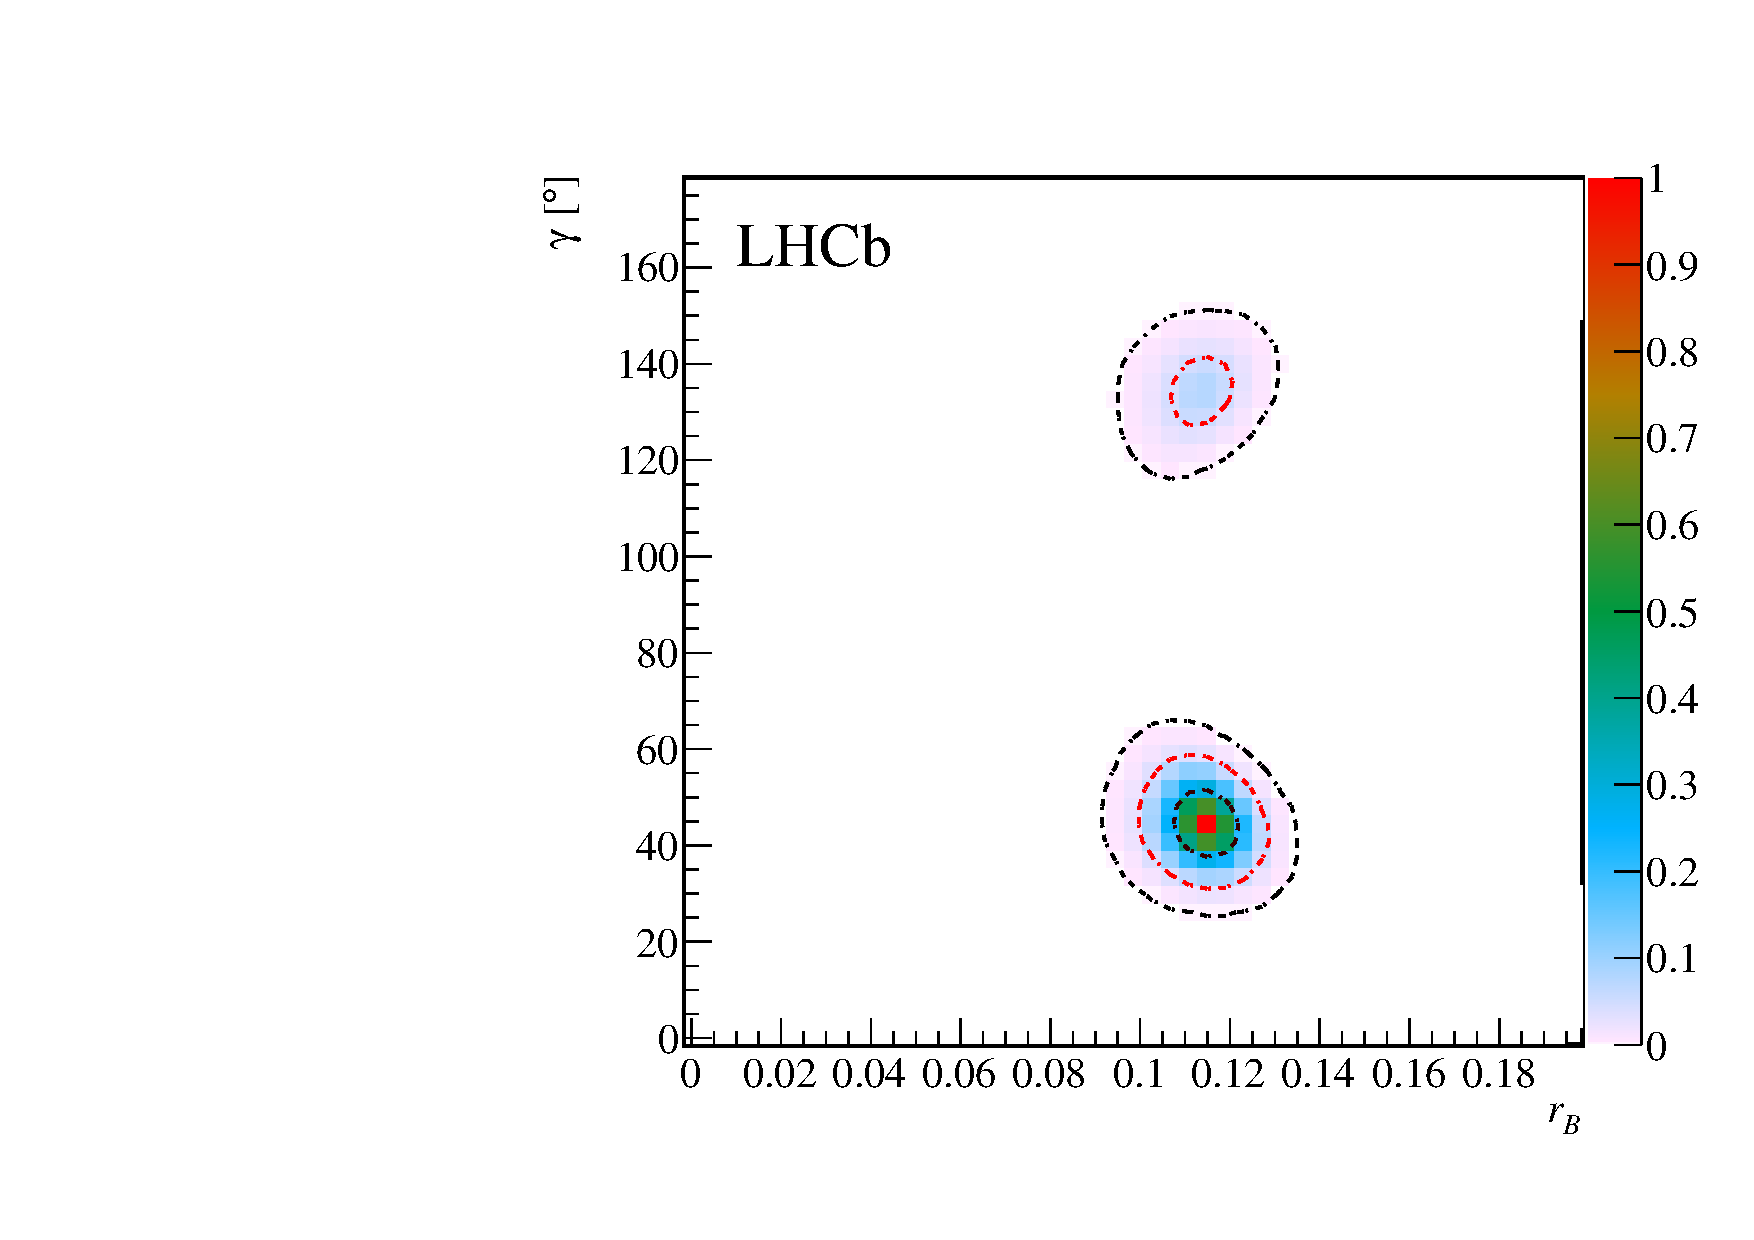
\includegraphics[width=0.5\linewidth]{figures/interpretation/rBu_dkstar_gamma_2Dscan_nomixing_Run3.pdf}}
\subfloat[\deltab versus \Pgamma]{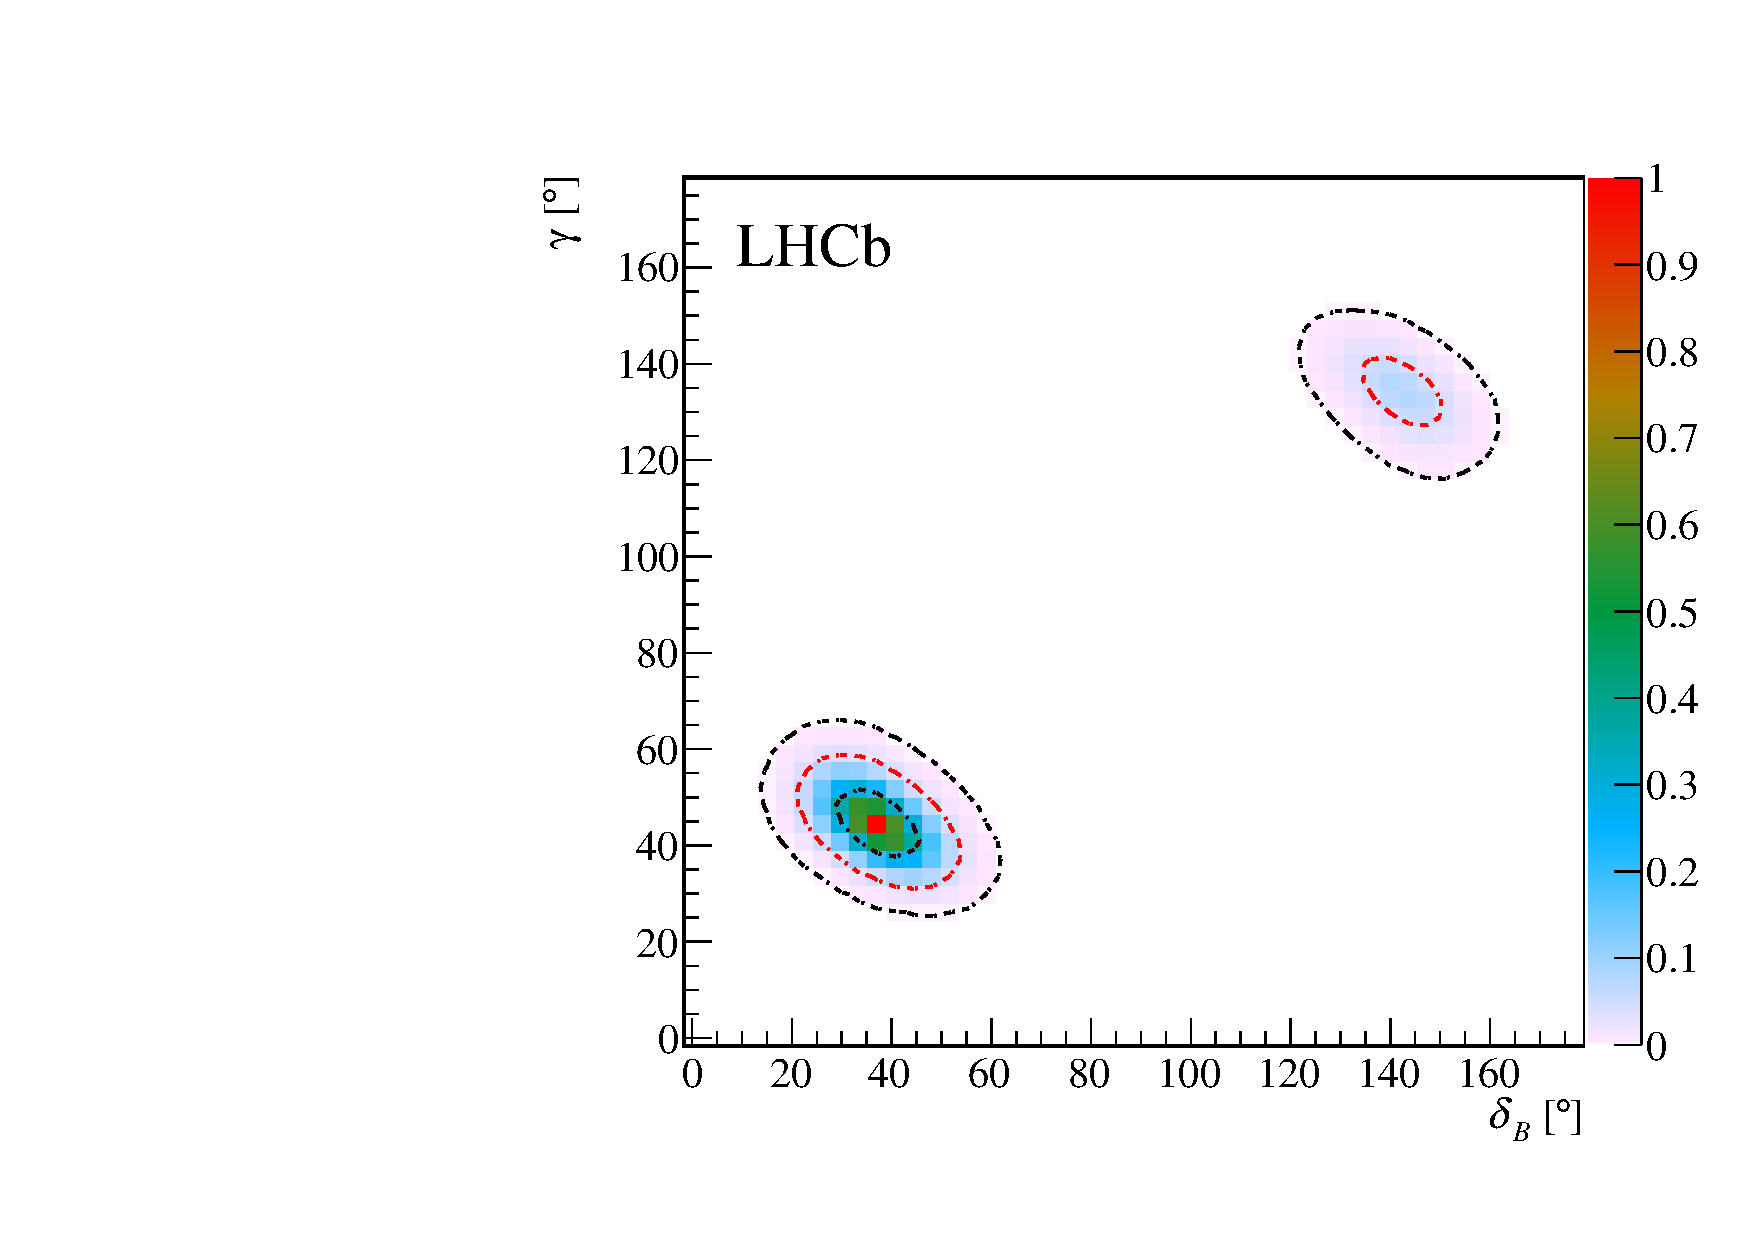
\includegraphics[width=0.5\linewidth]{figures/interpretation/deltaBu_dkstar_gamma_2Dscan_nomixing_Run3.pdf}}
\caption{Contour plots showing projected 2D scans of the physics parameters measured in \btodkst decays at the end of Run 3, assuming the central values remain the same. The dashed lines represent the $\Delta \chi^2 = 2.30,\ 6.18,\ \text{and } 11.8$ contours, corresponding to 68.3\%, 95.5\%, and 99.7\% CL, respectively. The colour scale represents $(1 - \text{CL})$.}
\label{gammadiniplotsrun3}
\end{figure}

It can be seen that the sensitivity of \rb, \deltab and \Pgamma continues to improve significantly with more data since the uncertainties are dominated by statistical uncertainty; therefore the \btodkst channel will continue to benefit from the increased dataset in Run 3 and beyond. At the end of Run 3 the uncertainty on \Pgamma, from \btodkst decays as investigated in this thesis, is expected to reduce to about $5^{\circ}$. Uncertainties in the measurements of the hadronic parameters in \btodkst decays, \rb and \deltab, will also reduce significantly to about $0.006$ and $7^{\circ}$ respectively. However, \fig\ref{gammadiniplotsrun3} demonstrates that even with these additional data, multiple solutions will exist. This problem of multiple solutions can be resolved by investigating alternative decays of the \Dz meson via the GGSZ method~\cite{GGSZ}, which involves analysing \Dz decays to \KS\pip\pim and \KS\Kp\Km final states~\cite{LHCb-PAPER-2012-027,LHCb-PAPER-2014-041}.

This thesis has presented the first \btodkst measurement at \lhcb and one of the first \CP violation measurements at \lhcb with Run 2 data. Additionally, the current world's best sensitivity to the hadronic parameters of the \Bm decay, \rb and \deltab, has been reported. There has been significant growth in understanding and interest with respect to amplitude analyses of \B decays. Independent information such as the measurements presented in this thesis, particularly on phases, is a significant asset to developing amplitude models. Further studies into \btodkst decays, subsequently leading to the development of an amplitude model for \decay{\Bm}{\D\KS\pim} decays, would provide a greater understanding of resonant structures present in the \KS\pim system. Such an investigation would benefit greatly from the parameters \rb and \deltab as constraints in the model, which can only be provided by studies of \btodkst decays as presented in this thesis. 

The suite of \Pgamma measurements is dominated, and will continue to be dominated, by \decay{\Bm}{\D\Km} measurements~\cite{LHCb-CONF-2017-004}. However, the analysis of the \decay{\Bm}{\D\Km} mode requires the modelling of several challenging backgrounds, most notably the misidentification background from \decay{\Bm}{\D\pim} decays and also partially reconstructed background, which both overlap with the signal region. Therefore, all \decay{\Bm}{\D\Km} measurements are accompanied by systematic uncertainties relating to these sources. Expanding the field of \Pgamma-sensitive measurements to include other \Bm decays, namely \decay{\Bm}{\D\Kstarm} decays, which contains relatively few challenging background components, provides an invaluable cross-check for the \Pgamma measurements made with \decay{\Bm}{\D\Km} decays. Hence future measurements of \decay{\Bm}{\D\Kstarm} decay modes are anticipated with significant interest.

The global strategy to measure \Pgamma in a wide variety of \B and \D decay modes is central to achieving the best precision of this parameter. The latest combination of results from a variety of \Pgamma-sensitive analyses at \lhcb gives a measurement of $\left(76.8^{+5.1}_{-5.7}\right)^{\circ}$~\cite{LHCb-CONF-2017-004}, which includes preliminary results from the work in this thesis. Different methods have been developed to investigate a range of decays modes of the \Dz meson using the \decay{\Bm}{\D\Km} channel. The work presented in this thesis leads the way for a completely new, though physically similar, \decay{\Bm}{\D\Kstarm} channel to be exploited using the many different \D decay modes developed for the \decay{\Bm}{\D\Km} channel. This work opens the door for a whole new range of \Pgamma-sensitive analyses to be developed. Furthermore, the work in this thesis can be further expanded by considering \decay{\Bm}{\D\Kstarm} decays, where the \Kstarm meson is reconstructed as \Km\piz. The inclusion of this alternative mode would result in a gain in \Pgamma-sensitivity from the additional data. However, as mentioned previously, this mode is significantly more difficult to reconstruct.

Measurements of \Pgamma will continue in the future, using as much data and as many \B and \D modes as possible, in order to reduce the statistical uncertainty. The expected sensitivity of \Pgamma at the end of Run 2 is $4^{\circ}$~\cite{LHCb-PAPER-2012-031}. The upgrade of Run 3 and beyond is estimated to provide a luminosity of 50~\invfb by the end of 2030, and achieve a significant increase in signal efficiency for \B meson decays, resulting in a predicted sensitivity to \Pgamma of $0.9^{\circ}$~\cite{LHCb-PAPER-2012-031}. Additionally, the Belle II experiment, which is expecting to collect a data sample corresponding to an integrated luminosity of 50~$\text{ab}^{\text{-1}}$ between 2018 and 2026, predicts a determination of \Pgamma to $1.6^{\circ}$~\cite{BelleII}. The \decay{\Bm}{\D\Kstarm(\KS\pim)} decay mode will have a relatively higher power for measuring \Pgamma at Belle II as the \KS reconstruction efficiency will be much improved compared to \lhcb. By continuing to measure \Pgamma in many different \B and \D modes, benefiting from the \btodkst channel introduced in this thesis and making full use of the increasing amount of data available, the Standard Model will be probed to unprecedented levels of precision. Through these multitude of measurements, it is hoped that signs of New Physics will begin to emerge.

\clearpage